\section{Models of product differentiation as random utility models}\label{sec:06-models}

The random utility model of \cref{sec:06-rum} is a general language for demand. A model of product
differentiation fills in two objects of that language. The first is the utility function
$U(x_j, p_j, \xi_j, \nu_i; \theta)$. The second is the distribution $F$ of the consumer tastes $\nu_i$. The
classical models of the theory literature (address models, ideal-point models, vertical models) and the
logit-type models of empirical work differ only in these two choices. This section places them in one
framework. The comparison matters because each specification fixes, before any data are used, which
products compete with which. Those restrictions drive every counterfactual the model produces.
\Cref{tab:06-taxonomy} at the end of the section collects the comparison.

\subsection{Horizontal and vertical differentiation}\label{sec:06-horvert}

Products are \emph{differentiated} when consumers do not regard them as perfect substitutes. Two polar
forms of differentiation organize the theory. They differ in whether consumers agree on how to rank the
products when prices are equal.

\begin{definition}[Vertical and horizontal differentiation]\label{def:06-vertical}
Let a consumer of type $\nu$ obtain utility $U(x_j, p, \nu)$ from product $j$ sold at price $p$. The
products are \emph{vertically differentiated} if at any common price every consumer ranks them in the
same order. Formally, for all products $j$ and $k$, all prices $p$, and all types $\nu$ and $\nu'$,
\begin{equation*}
  U(x_j, p, \nu) > U(x_k, p, \nu) \iff U(x_j, p, \nu') > U(x_k, p, \nu').
\end{equation*}
The products are \emph{horizontally differentiated} if at some common price two types rank some pair of
products differently.
\end{definition}

Under vertical differentiation a scalar index summarizes the common ranking. We call it \emph{quality}
and write it $\delta_j$. Consumers agree that higher quality is better. They disagree only about how much
extra money the extra quality is worth. Under horizontal differentiation no such index exists. At the same
price some consumers prefer a sweetened breakfast cereal and others a plain one, and neither group is
mistaken. Most markets mix the two forms. Every buyer prefers a luxury sedan to an economy sedan at the
same price, while buyers disagree about a sedan and a pickup truck.

The models below share a property that makes their demand systems tractable when tastes are
one-dimensional.

\begin{definition}[Single crossing]\label{def:06-singlecrossing}
Let the type $\nu$ be a scalar. Utility has the \emph{single-crossing property} if, for every pair of
products $j \ne k$ and all prices, the difference $U(x_j, p_j, \nu) - U(x_k, p_k, \nu)$ changes sign at
most once as $\nu$ increases. A sufficient condition is that the difference be strictly monotone in $\nu$.
\end{definition}

Under single crossing the utilities of two products, viewed as functions of the type, cross at most once.
The types that prefer $j$ to $k$ then form a half-line. The types that choose $j$ from the whole menu
form an interval, the intersection of such half-lines. Market shares become differences of the CDF $F$
evaluated at interval end points. Both the Hotelling model with quadratic transport costs and the
vertical model have this property. It is the reason their demand systems have closed forms, and the
reason each product competes only with its immediate neighbors.

\subsection{Address models: Hotelling and Salop}\label{sec:06-hotelling}

In an \emph{address model} each product has a location $x_j$ in a space of characteristics, and each
consumer has an ideal location in the same space. A consumer who buys a product away from her ideal
suffers a disutility that rises with the distance. \citet{Hotelling1929} introduced the idea with
consumers spread along a line. In random utility form, with quadratic distance costs,
\begin{equation}\label{eq:06-hotelling-u}
  u_{ij} = \bar u + (y_i - p_j) - \tau\, d(x_j, \nu_i)^2,
\end{equation}
where $\bar u$ is a utility constant common to all consumers, $y_i$ is income, $\nu_i$ is the consumer's
ideal location, and $d$ is distance. The coefficient $\tau > 0$ is the \emph{transport cost}. We reserve
$\theta$ for the generic parameter vector of \cref{sec:06-rum}, so the transport cost is always $\tau$.
The taste $\nu_i$ is now a location, and its distribution $F$ plays the role that the error distribution
plays in an additive random utility model. Products are horizontally differentiated. At equal prices
each consumer ranks products by distance, and consumers at different locations disagree.

\begin{example}[Hotelling duopoly with quadratic transport costs]\label{ex:06-hotelling}
Two firms sit at the ends of the unit interval, $x_1 = 0$ and $x_2 = 1$, and produce at common marginal
cost $c$. A mass $M$ of consumers is uniform on $[0,1]$, so $F(\nu) = \nu$. A consumer who buys nothing
obtains $y_i$. We assume $\bar u$ is large enough that every consumer buys one unit (full coverage).
Income and $\bar u$ then enter both inside utilities and cancel from the comparison.

The first step finds the indifferent consumer. A consumer at $\nu$ prefers firm 1 if
$-p_1 - \tau\nu^2 > -p_2 - \tau(1-\nu)^2$. The indifferent type $\nu^*$ solves
\begin{align*}
  p_1 + \tau(\nu^*)^2 &= p_2 + \tau(1-\nu^*)^2,\\
  \tau\big[(\nu^*)^2 - (1-\nu^*)^2\big] &= p_2 - p_1,\\
  \tau(2\nu^* - 1) &= p_2 - p_1,
\end{align*}
so that
\begin{equation}\label{eq:06-hotelling-cut}
  \nu^* = \frac{1}{2} + \frac{p_2 - p_1}{2\tau}.
\end{equation}
The utility difference $u_{i1} - u_{i2} = p_2 - p_1 + \tau(1 - 2\nu_i)$ falls in $\nu_i$ (single
crossing), so every consumer to the left of $\nu^*$ buys from firm 1.

The second step writes demand. Firm 1 sells $q_1 = M F(\nu^*) = M\nu^*$ and firm 2 sells
$q_2 = M(1 - \nu^*)$. These formulas hold when $0 < \nu^* < 1$, that is, when $|p_2 - p_1| < \tau$.
Demand is linear in prices, with $\frac{\partial q_1}{\partial p_1} = -\frac{M}{2\tau}$.

The third step finds best responses. Firm 1 maximizes $\pi_1 = (p_1 - c)M\nu^*(p_1, p_2)$, a concave
quadratic in $p_1$. Its first-order condition is
\begin{equation*}
  M\Big[\nu^* - \frac{p_1 - c}{2\tau}\Big] = 0.
\end{equation*}
Substituting \eqref{eq:06-hotelling-cut} gives $\frac{1}{2} + \frac{p_2 - p_1}{2\tau} = \frac{p_1 - c}{2\tau}$.
Multiplying by $2\tau$ and collecting terms gives the best response
\begin{equation*}
  p_1 = \frac{p_2 + c + \tau}{2}.
\end{equation*}

The fourth step imposes symmetry. With $p_1 = p_2 = p$, the best response becomes $p = \frac{p + c + \tau}{2}$,
so
\begin{equation}\label{eq:06-hotelling-eq}
  p_1 = p_2 = c + \tau, \qquad \nu^* = \frac{1}{2}, \qquad \pi_1 = \pi_2 = \frac{M\tau}{2}.
\end{equation}
The markup equals the transport cost. As $\tau \to 0$ the two products become perfect substitutes and
the price falls to marginal cost, the Bertrand outcome of \cref{ch:theory}. Full coverage holds in this
equilibrium when the consumer at $\nu = \frac{1}{2}$ prefers buying, $\bar u - c - \tau - \frac{\tau}{4}
\ge 0$, that is, $\bar u \ge c + \frac{5\tau}{4}$. The equilibrium is the case $x_1 = 0$, $x_2 = 1$ of
\cref{prop:04-hotelling}. Linear transport costs with the firms at the end points give the same indifferent
consumer and the same prices (\cref{sec:04-hotelling-linear}).
\end{example}

The quadratic form of the transport cost keeps demand continuous. With linear costs
$\tau\, d(x_j, \nu_i)$, demand jumps when one firm cuts its price far enough below its rival's to capture
the consumers at the rival's own location. \citet{DAspremontGabszewiczThisse1979} show that no pure-strategy
price equilibrium then exists when the two firms are located near the center of the line at distinct points
(\cref{prop:04-dgt}). With quadratic costs a price equilibrium exists for every pair of locations. In the two-stage game in which firms first choose locations and then prices, the firms move to
the two ends of the line, because distance softens price competition. \Cref{prop:04-hotelling} derives this
maximal differentiation in the location stage, and \cref{sec:04-hotelling-quad} shows that it exceeds the
efficient differentiation.

\citet{Salop1979} removed the end points of the line by placing consumers on a circle. Consider $N$ firms
spaced evenly on a circle of circumference one, each with marginal cost $c$. Transport cost is linear with
coefficient $\tau$. A mass $M$ of consumers is uniform on the circle, and every consumer buys. Take a firm that
charges $p$ while its two neighbors, each at distance $\frac{1}{N}$, charge $\bar p$. A consumer at distance $z$
from the firm, on the arc toward a neighbor, is indifferent when
\begin{equation*}
  p + \tau z = \bar p + \tau\Big(\frac{1}{N} - z\Big),
  \qquad\text{so}\qquad
  z = \frac{1}{2N} + \frac{\bar p - p}{2\tau}.
\end{equation*}
The firm serves consumers on both arcs, so its demand is
\begin{equation*}
  q = 2Mz = M\Big[\frac{1}{N} + \frac{\bar p - p}{\tau}\Big] \qquad\text{for } |\bar p - p| \le \frac{\tau}{N}.
\end{equation*}
Demand depends on the prices of the two neighbors and on no other price. By \cref{prop:04-salop}, the symmetric
equilibrium price is $p = c + \frac{\tau}{N}$, so the markup falls as products crowd the circle. With a fixed cost
of entry, free entry yields twice the efficient number of firms. Every consumer buys, so the markup is a
transfer, and the only distortion is in the number of firms. An entrant takes business from its neighbors,
while society gains only the saving in transport costs \citep[sec.~7.1.2]{Tirole1988}. Entry remains excessive
with quadratic transport costs (\cref{sec:04-salop}). Each firm in the Salop model competes only with its two
neighbors, a feature it shares with the vertical model below.

\subsection{The ideal-point model}\label{sec:06-idealpoint}

The address model extends to $K$ characteristics. In the \emph{ideal-point model}
\citep{AndersonDePalmaThisse1992} consumer $i$ has an ideal level $\nu_{ik}$ of each characteristic $k$,
and utility is
\begin{equation}\label{eq:06-idealpoint}
  u_{ij} = f(y_i, p_j) + \delta_j - \sum_{k=1}^K \alpha_k (x_{jk} - \nu_{ik})^2, \qquad \alpha_k > 0.
\end{equation}
Here $f(y_i, p_j)$ is the utility of the income left after the purchase, with $f_y > 0$, $f_p < 0$ and
$f_{py} \ge 0$ as in \cref{sec:06-normalization}. The term $\delta_j$ is a product effect common to all
consumers, and $\alpha_k$ is the weight of distance along dimension $k$. We write the distance term with
a minus sign and positive weights, so that utility falls with distance.\footnote{Some presentations
write the distance term with a plus sign. The weights must then be negative for distance to be costly.
We use the minus sign with positive weights.} The next result shows that
the ideal-point model is a special case of the pure characteristics model introduced below.

\begin{proposition}[Ideal points are random coefficients]\label{prop:06-idealpoint}
Under \eqref{eq:06-idealpoint},
\begin{equation}\label{eq:06-idealpoint-expanded}
  u_{ij} = f(y_i, p_j) + \Big[\delta_j - \sum_{k=1}^K \alpha_k x_{jk}^2\Big]
           + \sum_{k=1}^K 2\alpha_k\nu_{ik}\, x_{jk} - \sum_{k=1}^K \alpha_k\nu_{ik}^2 .
\end{equation}
Consequently, the following hold.
\begin{enumerate}[label=(\roman*)]
  \item Comparisons among inside products depend on the tastes only through the interactions
        $\nu_{ik}x_{jk}$. The model is a random coefficients model without an idiosyncratic shock. Its mean
        utility is $\delta_j - \sum_k \alpha_k x_{jk}^2$, and characteristic $x_{jk}$ carries the random
        coefficient $2\alpha_k\nu_{ik}$.
  \item The term $-\sum_k \alpha_k\nu_{ik}^2$ is the same for every inside product, so it cancels from
        every comparison among them. Relative to an outside good with utility $f(y_i, 0)$, it acts as a
        random coefficient on a characteristic that equals one for every inside product.
\end{enumerate}
\end{proposition}

\begin{proof}
Expand each square:
\begin{equation*}
  (x_{jk} - \nu_{ik})^2 = x_{jk}^2 - 2x_{jk}\nu_{ik} + \nu_{ik}^2 .
\end{equation*}
Multiply by $-\alpha_k$ and sum over $k$:
\begin{equation*}
  -\sum_k \alpha_k (x_{jk} - \nu_{ik})^2 = -\sum_k \alpha_k x_{jk}^2 + \sum_k 2\alpha_k\nu_{ik}x_{jk}
  - \sum_k \alpha_k\nu_{ik}^2 .
\end{equation*}
Substituting into \eqref{eq:06-idealpoint} gives \eqref{eq:06-idealpoint-expanded}. For two inside
products $j$ and $l$,
\begin{equation*}
  u_{ij} - u_{il} = f(y_i, p_j) - f(y_i, p_l) + \Big[\delta_j - \sum_k \alpha_k x_{jk}^2\Big]
  - \Big[\delta_l - \sum_k \alpha_k x_{lk}^2\Big] + \sum_k 2\alpha_k\nu_{ik}(x_{jk} - x_{lk}),
\end{equation*}
in which $\nu_{ik}^2$ no longer appears. This proves (i) and the first part of (ii). The difference
$u_{ij} - u_{i0}$ keeps the term $-\sum_k \alpha_k\nu_{ik}^2$, which is the product of a consumer-specific
coefficient and the constant one. This proves the rest of (ii).
\end{proof}

\citet[eq.~6]{BerryPakes2007} make the same point. They write the ideal-point model with a distance
between the consumer's location and the product's location. With Euclidean distance, they note, expanding
the squares leaves a mean utility that depends on characteristics. The individual term is then built from
interactions of consumer and product characteristics. The quadratic term
$-\alpha_k x_{jk}^2$ in mean utility is what distinguishes ideal points from linear random coefficients.
It makes the value of a characteristic peak at the consumer's ideal and decline beyond it. With linear
random coefficients and tastes $\nu_{ik}$ of both signs, consumers also disagree about the direction in
which a characteristic is good, which is another form of horizontal differentiation.

\subsection{Two families of empirical models}\label{sec:06-classes}

The empirical models of this book fall into two families. The first is the \emph{pure characteristics
model} \citep{BerryPakes2007}, in which consumers have tastes for characteristics and for nothing else:
\begin{equation}\label{eq:06-pc-class}
  u_{ij} = f(y_i, p_j) + \delta_j + \sum_{k=1}^K \sigma_k \nu_{ik} x_{jk}.
\end{equation}
Here $\nu_{ik}$ is a standardized taste for characteristic $k$ and $\sigma_k \ge 0$ its dispersion, the
$k$-th diagonal element of the matrix $\Sigma$ in the random coefficients notation of \cref{ch:blp}. The
model is also called the \emph{pure hedonic} model. By \cref{prop:06-idealpoint}, the ideal-point model
belongs to this family once its quadratic terms are counted among the characteristics and a constant
inside-good characteristic is added. The second family adds an idiosyncratic shock $\epsilon_{ij}$:
\begin{equation}\label{eq:06-blp-class}
  u_{ij} = f(y_i, p_j) + \delta_j + \sum_{k=1}^K \sigma_k \nu_{ik} x_{jk} + \epsilon_{ij},
\end{equation}
with $\epsilon_{ij}$ i.i.d.\ across products and consumers. With type-I extreme value shocks this is the
random coefficients logit model of \citet{BerryLevinsohnPakes1995}, the subject of \cref{ch:blp}. With
$\sigma_k = 0$ for all $k$ it is the logit model of \cref{sec:06-tiev}.

The function $f$ carries income effects. In the quasi-linear case $f(y_i, p_j) = \alpha(y_i - p_j)$ income
enters every alternative equally and cancels, and the price coefficient $\alpha$ is common to all
consumers. \citet{BerryLevinsohnPakes1995} use $f(y_i, p_j) = \alpha\ln(y_i - p_j)$, which makes richer
consumers less price sensitive ($f_{py} > 0$). The properties of $f$ are derived in
\cref{sec:06-normalization}.

The key difference between \eqref{eq:06-pc-class} and \eqref{eq:06-blp-class} is the shock
$\epsilon_{ij}$. With $\epsilon_{ij}$ in the model, the product space can never be exhausted. Each new
product arrives with a fresh draw of $\epsilon_{ij}$ for every consumer, which guarantees it a positive
share and some market power wherever it is placed. In the pure characteristics model a new product placed
next to an existing one is a near-perfect substitute for it. \Cref{sec:06-epsilon} develops the
consequences for markups and for the welfare value of new products. The vertical model, to which we now
turn, is the pure characteristics model with a single characteristic, quality, and a single random
coefficient, on price.

\subsection{The vertical model as a random utility model}\label{sec:06-vdef}

The \emph{vertical model} specifies
\begin{equation}\label{eq:06-vertical-u}
  u_{ij} = \delta_j - \nu_i p_j, \qquad \nu_i > 0,
\end{equation}
with outside good $u_{i0} = 0$. The products are vertically differentiated in the sense of
\cref{def:06-vertical}. At any common price $p$, $u_{ij} - u_{ik} = \delta_j - \delta_k$ for every consumer,
so all consumers rank products by $\delta_j$. Consumers differ only in their \emph{price sensitivity}
$\nu_i$, the utility cost of a dollar. A consumer with high $\nu_i$ dislikes paying and buys cheap,
low-quality products. A consumer with low $\nu_i$ pays a lot for quality. The cabins of an airline (first,
business, economy) fit this description. Every traveler prefers the front cabin at equal prices, and
travelers sort across cabins by willingness to pay. Storage or memory tiers of an otherwise identical device are a
second example.

Dividing \eqref{eq:06-vertical-u} by $\nu_i > 0$ gives an equivalent form. With $v_i = \frac{1}{\nu_i}$,
\begin{equation}\label{eq:06-vertical-v}
  \frac{u_{ij}}{\nu_i} = v_i\delta_j - p_j .
\end{equation}
Here $v_i$ is the consumer's willingness to pay for a unit of quality. A consumer-specific positive
rescaling of utility leaves choices unchanged (\cref{sec:06-normalization}), so the two forms imply the
same demand. The form \eqref{eq:06-vertical-v} is the one used by \citet{MussaRosen1978} and by
\citet{Bresnahan1987}, who attributes the demand system to \citet{PrescottVisscher1977}. In this form the
consumer buys the product with the lowest ``total price'' $p_j - v_i\delta_j$.

The vertical model has the single-crossing property. For two products with $p_k > p_j$,
\begin{equation}\label{eq:06-vertical-sc}
  u_{ij} - u_{ik} = (\delta_j - \delta_k) + \nu_i(p_k - p_j)
\end{equation}
is strictly increasing in $\nu_i$. The preference for the cheaper product rises with price sensitivity.
More generally, consider any model with a scalar type in which all consumers agree on the quality ranking.
It is vertical and single crossing whenever the marginal rate of substitution between quality and money
is monotone in the type. \citet{GabszewiczThisse1979} obtain such a model from income differences. In their specification
$u_{ij} = \delta_j(y_i - p_j)$, and a consumer with income $y$ prefers $j$ to $k$ (with $\delta_j > \delta_k$
and $p_j > p_k$) if and only if
\begin{equation*}
  \delta_j(y - p_j) > \delta_k(y - p_k)
  \iff y(\delta_j - \delta_k) > \delta_j p_j - \delta_k p_k
  \iff y > \frac{\delta_j p_j - \delta_k p_k}{\delta_j - \delta_k} .
\end{equation*}
Richer consumers buy higher quality, and the cutoffs now live in income space. \citet{ShakedSutton1982}
embed this demand system in a two-stage game. Firms first choose qualities and then compete in prices,
and in equilibrium they choose distinct qualities to relax price competition. \citet{MussaRosen1978}
study a monopolist that offers a menu of qualities to consumers with utility $v_i\delta - p$. The
monopolist screens consumers by quality and supplies every type except the highest a quality below the
efficient level. These theory results take the vertical structure as given. \Cref{sec:06-vertical}
develops its demand side for estimation.

\subsection{The logit as a model of differentiation}\label{sec:06-logitdiff}

The logit model $u_{ij} = \delta_j - \alpha p_j + \epsilon_{ij}$, with $\epsilon_{ij}$ i.i.d.\ type-I extreme
value (\cref{prop:06-logit}), is also a model of differentiation. Each product carries its own taste
dimension. \Cref{rem:06-tastesforproducts} reads the shock $\epsilon_{ij}$ as consumer $i$'s random taste for
a characteristic that only product $j$ possesses, the product's own dummy variable. Under this reading, which
\citet{BerryPakes2007} attribute to \citet{CaplinNalebuff1991}, the characteristic space of the logit has one
dimension per product. Adding a product adds a dimension, so every product owns a
neighborhood of taste space that no rival can enter. This is the formal content of the statement that
the product space is never exhausted.

The logit treats every pair of products as equally distant. Consumers who leave a product spread over the
others in proportion to their shares, the independence of irrelevant alternatives property examined in
\cref{sec:06-gev} and \cref{ch:logit}. \citet{AndersonDePalmaThisse1989} give the logit a deterministic address
representation, with no random utility shock. Their consumers have ideal points as in \eqref{eq:06-idealpoint}, with
utility linear in price and a common weight on every characteristic. With $J$ products and no outside good, each
demand rises strictly with every rival price, at every price vector, only if the products span at least $J-1$
dimensions \citep[Proposition~1]{AndersonDePalmaThisse1989}. We follow \citet{AndersonDePalmaThisse1989} and place
product $J$ at the origin and each product $j<J$ at the same distance along the axis of characteristic $j$. These
locations span exactly $J-1$ dimensions. We also give the products equal quality. Logit demand then arises from a
unique density of ideal points, which has a single peak at the point equidistant from all products
\citep[Propositions~2 and~4]{AndersonDePalmaThisse1989}. Other locations that span $J-1$ dimensions also give a
unique density, though a different one \citep[p.~26]{AndersonDePalmaThisse1989}.
The nested logit adds a taste common to the products of a group, and the random coefficients logit adds
tastes for characteristics. Both keep the product-specific shock. \Cref{tab:06-taxonomy} summarizes how
the models differ.

\begin{table}[htbp]
\centering
\caption{Discrete choice models of product differentiation compared}\label{tab:06-taxonomy}
\footnotesize
\renewcommand{\arraystretch}{1.3}
\begin{tabularx}{\textwidth}{@{}>{\raggedright\arraybackslash}p{3.0cm}>{\raggedright\arraybackslash}p{1.55cm}>{\raggedright\arraybackslash}X>{\raggedright\arraybackslash}p{1.1cm}>{\raggedright\arraybackslash}p{2.05cm}>{\raggedright\arraybackslash}p{2.0cm}@{}}
\toprule
Model and utility & Dimension of heterogeneity & Who substitutes with whom & Closed-form shares & Markups as products crowd the space & Surplus from an added clone \\
\midrule
Hotelling, Salop\newline $-p_j - \tau\, d(x_j,\nu_i)^2$ & 1 (location) & Neighbors on the line or circle & Yes & Fall to zero ($\frac{\tau}{N}$ in Salop) & Zero \\
Ideal point\newline $\delta_j - p_j$\newline $-\sum_k \alpha_k(x_{jk}-\nu_{ik})^2$ & $K$ (ideal points) & Products close in characteristic space & No & Fall to zero & Zero \\
Pure characteristics\newline $\delta_j - \alpha p_j + \sum_k \sigma_k\nu_{ik}x_{jk}$ & $K$ (tastes for characteristics) & Products close in characteristics and price & No & Fall to zero & Zero \\
Vertical\newline $\delta_j - \nu_i p_j$ & 1 (price sensitivity) & Price neighbors only & Yes & Fall to zero for neighbors owned by rivals & Zero \\
Logit\newline $\delta_j - \alpha p_j + \epsilon_{ij}$ & $J$ (one taste per product) & All products, in proportion to shares & Yes & Bounded below by $\frac{1}{\alpha}$ & Positive \\
Nested logit\newline $\delta_j - \alpha p_j + \zeta_{ig}$\newline $+\,(1-\sigma)\epsilon_{ij}$ & $J$ plus one per nest & Mostly within the nest, in proportion to shares & Yes & Bounded below by $\frac{1-\sigma}{\alpha}$ & Positive \\
Random coefficients logit\newline $\delta_j - \alpha p_j + \sum_k \sigma_k\nu_{ik}x_{jk}$\newline $+\,\epsilon_{ij}$ & $K$ plus $J$ & Mostly toward products with similar characteristics & No & Bounded away from zero & Positive \\
\bottomrule
\end{tabularx}
\par\smallskip
\begin{minipage}{\textwidth}
\footnotesize Notes: Utilities omit income, which cancels under quasi-linearity. $\tau$ is the transport cost,
$d$ a distance, $\nu_i$ the consumer's type, and $\sigma_k$ the dispersion of the taste for characteristic
$k$. In the nested logit, $\sigma \in [0,1)$ is the nesting parameter and $\zeta_{ig}$ is a taste for nest $g$
whose distribution makes $\zeta_{ig} + (1-\sigma)\epsilon_{ij}$ type-I extreme value. Markup bounds are for single-product
firms facing an outside good. ``Surplus from an added clone'' is the gain in expected consumer surplus,
at fixed prices, from adding an exact copy of an existing product. \Cref{sec:06-epsilon} derives the logit
entries, and \cref{ch:logit,ch:blp} treat the nested and random coefficients logit.
\end{minipage}
\end{table}

\section{The vertical model}\label{sec:06-vertical}

The vertical model is the simplest model in characteristic space that delivers closed-form demand, an
exact inversion from market shares to qualities, and a transparent supply side. It is the demand system of
the first structural test of conduct in a differentiated-products industry \citep{Bresnahan1987}, the
case study of \cref{sec:06-bresnahan}. It is also the building block from which \citet{BerryPakes2007}
compute shares in the pure characteristics model (\cref{sec:06-purechar}). This section develops the
model for a general taste distribution $F$, then specializes to exponential and uniform tastes. Every
derivation is carried out in the notation of \eqref{eq:06-vertical-u}.

\subsection{Setup and the ordering of products}\label{sec:06-vsetup}

\begin{assumption}[Vertical model]\label{ass:06-vertical}
\leavevmode
\begin{enumerate}[label=(\roman*)]
  \item A market has $M$ consumers and $J$ inside products. Consumer $i$ obtains $u_{ij} = \delta_j - \nu_i p_j$
        from product $j$, where $\delta_j$ is the product's quality and $p_j > 0$ its price.
  \item The outside good $j = 0$ has $\delta_0 = p_0 = 0$, so $u_{i0} = 0$.
  \item The price sensitivities $\nu_i$ are i.i.d.\ draws from a distribution with continuous and strictly
        increasing CDF $F$ on $(0,\infty)$ and density $f = F' > 0$. We set $F(x) = 0$ for $x \le 0$.
  \item Each consumer buys one unit of the product with the highest utility.
  \item Inside prices are distinct.
\end{enumerate}
\end{assumption}

Part (iii) makes ties a probability-zero event, so choices are well defined for almost every consumer. The
quality $\delta_j$ summarizes everything consumers value about product $j$, observed and unobserved. In
estimation we write $\delta_j = x_j\beta + \xi_j$. Part (v) is generic. If two products had the same price,
every consumer would buy the higher-quality one, and the other would sell nothing. The price sensitivity
is the only dimension of consumer heterogeneity. Consumers agree on how characteristics combine into
quality and disagree only on the marginal utility of money.

\begin{lemma}[Ordering]\label{lem:06-ordering}
Under \cref{ass:06-vertical}, if $p_j > p_k$ and product $j$ sells a positive quantity, then
$\delta_j > \delta_k$. Hence the products with positive sales, together with the outside good, can be
indexed so that
\begin{equation}\label{eq:06-ordering}
  0 = p_0 < p_1 < \dots < p_J \qquad\text{and}\qquad 0 = \delta_0 < \delta_1 < \dots < \delta_J .
\end{equation}
\end{lemma}

\begin{proof}
Suppose $p_j > p_k$ and $\delta_j \le \delta_k$. For every $\nu > 0$,
\begin{equation*}
  u_j(\nu) - u_k(\nu) = (\delta_j - \delta_k) - \nu(p_j - p_k) \le -\nu(p_j - p_k) < 0 .
\end{equation*}
Every consumer strictly prefers $k$ to $j$, so $j$ sells nothing. The contrapositive is the first claim.
Applying it with $k = 0$ shows that every product with positive sales has $\delta_j > 0$. Applying it to
every pair of products with positive sales orders their qualities as their prices.
\end{proof}

Among products that sell, price and quality rise together. A product that charges more than a rival and
offers less quality loses every consumer to that rival. We say it is \emph{dominated outright}. A subtler
form of domination is possible. A product can offer more quality than every cheaper product and still sell
nothing, because a combination of two rivals beats it for every consumer. The geometry of the
$(p, \delta)$ plane makes this precise.

\begin{proposition}[The quality-price frontier]\label{prop:06-frontier}
Let $\mathcal P = \{(p_0, \delta_0), (p_1, \delta_1), \dots, (p_J, \delta_J)\}$ be the points of the
$(p, \delta)$ plane occupied by the outside good and the $J$ products, with prices distinct but qualities
arbitrary. Under \cref{ass:06-vertical} the following hold.
\begin{enumerate}[label=(\roman*)]
  \item A consumer of type $\nu$ chooses product $j$ if and only if every other point of $\mathcal P$ lies
        strictly below the line through $(p_j, \delta_j)$ with slope $\nu$.
  \item Product $j \ge 1$ sells a positive quantity if and only if $(p_j, \delta_j)$ is a vertex of the
        \emph{quality-price frontier}. The frontier is the rising part of the upper boundary of the
        convex hull of $\mathcal P$.
  \item Equivalently, delete the products that sell nothing and index the rest by price. Then the slopes
        $\bar\nu_j = \frac{\delta_j - \delta_{j-1}}{p_j - p_{j-1}}$, $j = 1, \dots, J$, satisfy
        $\bar\nu_1 > \bar\nu_2 > \dots > \bar\nu_J > 0$.
\end{enumerate}
\end{proposition}

\begin{proof}
For (i), type $\nu$ chooses $j$ if and only if $\delta_j - \nu p_j > \delta_k - \nu p_k$ for all $k \ne j$.
Rearranging, this holds if and only if
\begin{equation*}
  \delta_k < \delta_j + \nu(p_k - p_j) \qquad \text{for all } k \ne j .
\end{equation*}
The right side is the height at $p_k$ of the line through $(p_j, \delta_j)$ with slope $\nu$.

For (ii), consider lines through $(p_j, \delta_j)$ that lie strictly above every other point of
$\mathcal P$. Such a line exists if and only if $(p_j, \delta_j)$ is a vertex of the upper boundary of the
convex hull of $\mathcal P$. Let $a_j$ be the slope of the hull edge to the left of that vertex. Let $b_j$ be
the slope of the edge to its right, with $b_j = -\infty$ at the right end of the hull. Concavity of the
upper boundary gives $a_j > b_j$. A line through the vertex lies strictly above all other points if and
only if its slope lies in the open interval $(b_j, a_j)$. By (i), the types that choose $j$ form the set
$(b_j, a_j) \cap (0, \infty)$. Because $F$ has a positive density on $(0,\infty)$, this set has positive
probability if and only if $a_j > 0$. In words, the vertex must lie on the rising part of the hull. The
share is then $F(a_j) - F(\max\{b_j, 0\})$. A point that lies on a hull edge without being a
vertex is chosen at most by the single type whose slope equals that edge's slope, a probability-zero
event.

For (iii), the products that sell are the vertices of the rising part of the hull. Indexed by price, the
edges between consecutive vertices have strictly decreasing slopes, because the upper boundary is
strictly concave at each vertex. The last slope is positive because the hull rises up to the
highest-quality product. Conversely, suppose the slopes of the chain through the remaining points are
positive and strictly decreasing. Then the chain is strictly concave and rising, so every point on it is a
vertex of the frontier.
\end{proof}

\Cref{fig:06-frontier} draws the frontier. The slopes of its edges are the \emph{cutoffs} studied in
\cref{sec:06-vcutoffs}. A product strictly below the frontier sells nothing. We say it is
\emph{dominated out of the market}. Two cases arise in the figure. Product $a$ is dominated outright by
product 1, which is cheaper and better. Product $b$ has more quality than every cheaper product, yet it
lies below the chord between products 2 and 3. Any consumer who would consider $b$ prefers either 2 or 3.
The frontier is computed by a scan over products sorted by price, the monotone-chain construction of the
convex hull.

\begin{enumerate}[label=Step \arabic*.,leftmargin=*]
  \item Sort the products by price and place the outside good $(0,0)$ first.
  \item Delete every product whose quality does not exceed the quality of every cheaper product, including
        the outside good. These products are dominated outright (\cref{lem:06-ordering}).
  \item Scan the remaining products in increasing order of price, keeping a list of frontier candidates
        that starts with the outside good. Before adding a new product, compare two slopes: the slope
        from the second-to-last candidate to the last, and the slope from the last candidate to the new
        product. If the first is less than or equal to the second, the last candidate lies on or below the
        chord, so delete it. Repeat the check until it fails, then add the new product.
  \item The final list is the frontier. Its products sell positive quantities, and the slopes between
        consecutive products are the cutoffs $\bar\nu_1 > \dots > \bar\nu_J$.
\end{enumerate}

\begin{figure}[htbp]
\centering
\begin{tikzpicture}[x=3cm,y=1.8cm,>=Stealth]
  \draw[->] (0,0) -- (3.75,0) node[below left] {price $p$};
  \draw[->] (0,0) -- (0,3.35) node[above] {quality $\delta$};
  \foreach \x/\y in {1/1.6, 2/2.4, 3.2/2.9} { \draw[densely dotted, gray] (\x,0) -- (\x,\y); }
  \node[below] at (1,0) {$p_1$};
  \node[below] at (2,0) {$p_2$};
  \node[below] at (3.2,0) {$p_3$};
  \draw (0,1.6) -- (-0.04,1.6) node[left] {$\delta_1$};
  \draw (0,2.4) -- (-0.04,2.4) node[left] {$\delta_2$};
  \draw (0,2.9) -- (-0.04,2.9) node[left] {$\delta_3$};
  \draw[very thick] (0,0) -- (1,1.6) -- (2,2.4) -- (3.2,2.9);
  \fill (0,0) circle (2pt) node[below right] {$0$};
  \fill (1,1.6) circle (2pt) node[above left] {$1$};
  \fill (2,2.4) circle (2pt) node[above left] {$2$};
  \fill (3.2,2.9) circle (2pt) node[above] {$3$};
  \draw[dashed, gray] (1,1.6) -- (1.62,1.6);
  \draw[thick, fill=white] (1.5,1.4) circle (2pt) node[below right] {$a$};
  \draw[thick, fill=white] (2.6,2.5) circle (2pt) node[below right] {$b$};
  \node[below right] at (0.5,0.78) {slope $\bar\nu_1$};
  \node[above left] at (1.47,2.0) {slope $\bar\nu_2$};
  \node[above] at (2.55,2.72) {slope $\bar\nu_3$};
\end{tikzpicture}
\caption{The quality-price frontier. Points are products in the $(p, \delta)$ plane, with the outside good
at the origin. The bold line is the rising part of the upper boundary of the convex hull, and its vertices
$1$, $2$ and $3$ are the products that sell. The slope of the edge ending at product $j$ is the cutoff
$\bar\nu_j = \frac{\delta_j - \delta_{j-1}}{p_j - p_{j-1}}$. Product $a$ is dominated outright by product 1
(higher price, lower quality). Product $b$ offers more quality than every cheaper product but lies below
the chord between products 2 and 3, so it sells nothing. The products are $(p_j, \delta_j) = (1, 1.6)$,
$(2, 2.4)$, $(3.2, 2.9)$, with $a = (1.5, 1.4)$ and $b = (2.6, 2.5)$.}
\label{fig:06-frontier}
\end{figure}

\subsection{Cutoffs and single crossing}\label{sec:06-vcutoffs}

From now on we index only the products on the frontier, in increasing order of price, as in
\eqref{eq:06-ordering}. A consumer compares each product first with its two price neighbors. She prefers
$j$ to the next more expensive product $j+1$ if and only if
\begin{align*}
  \delta_j - \nu p_j &> \delta_{j+1} - \nu p_{j+1}\\
  \iff \nu(p_{j+1} - p_j) &> \delta_{j+1} - \delta_j\\
  \iff \nu &> \frac{\delta_{j+1} - \delta_j}{p_{j+1} - p_j}.
\end{align*}
She prefers $j$ to the next cheaper product $j-1$ if and only if
\begin{align*}
  \delta_j - \nu p_j &> \delta_{j-1} - \nu p_{j-1}\\
  \iff \delta_j - \delta_{j-1} &> \nu(p_j - p_{j-1})\\
  \iff \nu &< \frac{\delta_j - \delta_{j-1}}{p_j - p_{j-1}}.
\end{align*}
Both thresholds are slopes of frontier edges. We define the \emph{cutoffs}
\begin{equation}\label{eq:06-cutoff}
  \bar\nu_j = \frac{\delta_j - \delta_{j-1}}{p_j - p_{j-1}}, \qquad j = 1, \dots, J,
  \qquad\text{with}\qquad \bar\nu_0 = \infty, \quad \bar\nu_{J+1} = 0 .
\end{equation}
The cutoff $\bar\nu_j$ is the type indifferent between $j-1$ and $j$. It measures the extra quality per
extra dollar gained by moving up from $j-1$ to $j$. In particular $\bar\nu_1 = \frac{\delta_1}{p_1}$ is the
type indifferent between buying product 1 and buying nothing. On the frontier the cutoffs are strictly
decreasing (\cref{prop:06-frontier}).

\begin{proposition}[Choice intervals]\label{prop:06-cutoffs}
Under \cref{ass:06-vertical}, let all $J$ products lie on the frontier, so that
$\bar\nu_1 > \bar\nu_2 > \dots > \bar\nu_J > 0$. Then consumer $i$ chooses product $j \in \{0, 1, \dots, J\}$
if and only if
\begin{equation}\label{eq:06-choice-interval}
  \bar\nu_{j+1} < \nu_i < \bar\nu_j .
\end{equation}
In particular, the two comparisons with the price neighbors are sufficient for the choice of $j$.
\end{proposition}

\begin{proof}
By \eqref{eq:06-vertical-sc}, for $k > j$ the difference $u_j(\nu) - u_k(\nu)$ is strictly increasing in $\nu$
(single crossing). The two equivalences above state that $j \succ j+1$ if and only if $\nu > \bar\nu_{j+1}$,
and $j \succ j-1$ if and only if $\nu < \bar\nu_j$.

Necessity. If $i$ chooses $j$, then $j$ beats both neighbors, so $\bar\nu_{j+1} < \nu_i < \bar\nu_j$. For
$j = 0$ only the comparison with product 1 applies, and it gives $\nu_i > \bar\nu_1$. For $j = J$ only the
comparison with $J - 1$ applies, and $\nu_i > 0 = \bar\nu_{J+1}$ holds by assumption.

Sufficiency. Suppose $\bar\nu_{j+1} < \nu_i < \bar\nu_j$. Consider first the more expensive products. For
every $m \ge j + 1$ the cutoffs decrease, so $\bar\nu_m \le \bar\nu_{j+1} < \nu_i$. Hence $m - 1 \succ m$ for
every such $m$, and the chain
\begin{equation*}
  u_j(\nu_i) > u_{j+1}(\nu_i) > \dots > u_J(\nu_i)
\end{equation*}
shows that $j$ beats every more expensive product. Consider next the cheaper products. For every
$m \le j$, $\bar\nu_m \ge \bar\nu_j > \nu_i$. Hence $m \succ m - 1$, and the chain
\begin{equation*}
  u_j(\nu_i) > u_{j-1}(\nu_i) > \dots > u_0(\nu_i)
\end{equation*}
shows that $j$ beats every cheaper product. Types exactly at a cutoff have probability zero.
\end{proof}

The proof uses the decreasing cutoffs at every step. If instead $\bar\nu_j \le \bar\nu_{j+1}$ for some $j$,
the interval in \eqref{eq:06-choice-interval} is empty and product $j$ sells nothing. In the $(p,\delta)$
plane such a product lies on or below the chord between $j - 1$ and $j + 1$, as \cref{prop:06-frontier}
says. Consumers sort by price sensitivity. The least price-sensitive consumers buy the top product, and
the most price-sensitive buy nothing. \Cref{fig:06-ulines} shows the construction with utility lines.

\begin{figure}[htbp]
\centering
\begin{subfigure}[b]{0.52\textwidth}
\centering
\begin{tikzpicture}[x=2.85cm,y=1.12cm,>=Stealth]
  \begin{scope}
    \clip (0,-0.35) rectangle (2.2,3.15);
    \draw[thin] (0,1.6) -- (2.2,-0.6);
    \draw[thin] (0,2.4) -- (1.7,-1.0);
    \draw[thin] (0,2.9) -- (1.21875,-1.0);
    \draw[thin, gray, dashed] (0,2.5) -- (1.3462,-1.0);
  \end{scope}
  \draw[->] (0,0) -- (2.3,0) node[below] {$\nu$};
  \draw[->] (0,-0.35) -- (0,3.25) node[above] {$u_j(\nu)$};
  \draw[very thick] (0,2.9) -- (0.416667,1.566667) -- (0.8,0.8) -- (1.6,0) -- (2.2,0);
  \node[left] at (0,1.6) {$\delta_1$};
  \node[left] at (0,2.4) {$\delta_2$};
  \node[left] at (0,2.92) {$\delta_3$};
  \draw (0,-0.85) -- (2.2,-0.85);
  \foreach \c in {0.416667, 0.8, 1.6} {
    \draw[densely dashed, gray] (\c,-0.85) -- (\c,{max(0,2.9-3.2*\c,2.4-2*\c,1.6-\c)});
    \draw (\c,-0.78) -- (\c,-0.92);
  }
  \draw (0,-0.78) -- (0,-0.92);
  \node[below] at (0.416667,-0.9) {$\bar\nu_3$};
  \node[below] at (0.8,-0.9) {$\bar\nu_2$};
  \node[below] at (1.6,-0.9) {$\bar\nu_1$};
  \node[above] at (0.208,-0.85) {\small $3$};
  \node[above] at (0.608,-0.85) {\small $2$};
  \node[above] at (1.2,-0.85) {\small $1$};
  \node[above] at (1.9,-0.85) {\small $0$};
\end{tikzpicture}
\caption{Utility lines and the upper envelope}
\end{subfigure}\hfill
\begin{subfigure}[b]{0.45\textwidth}
\centering
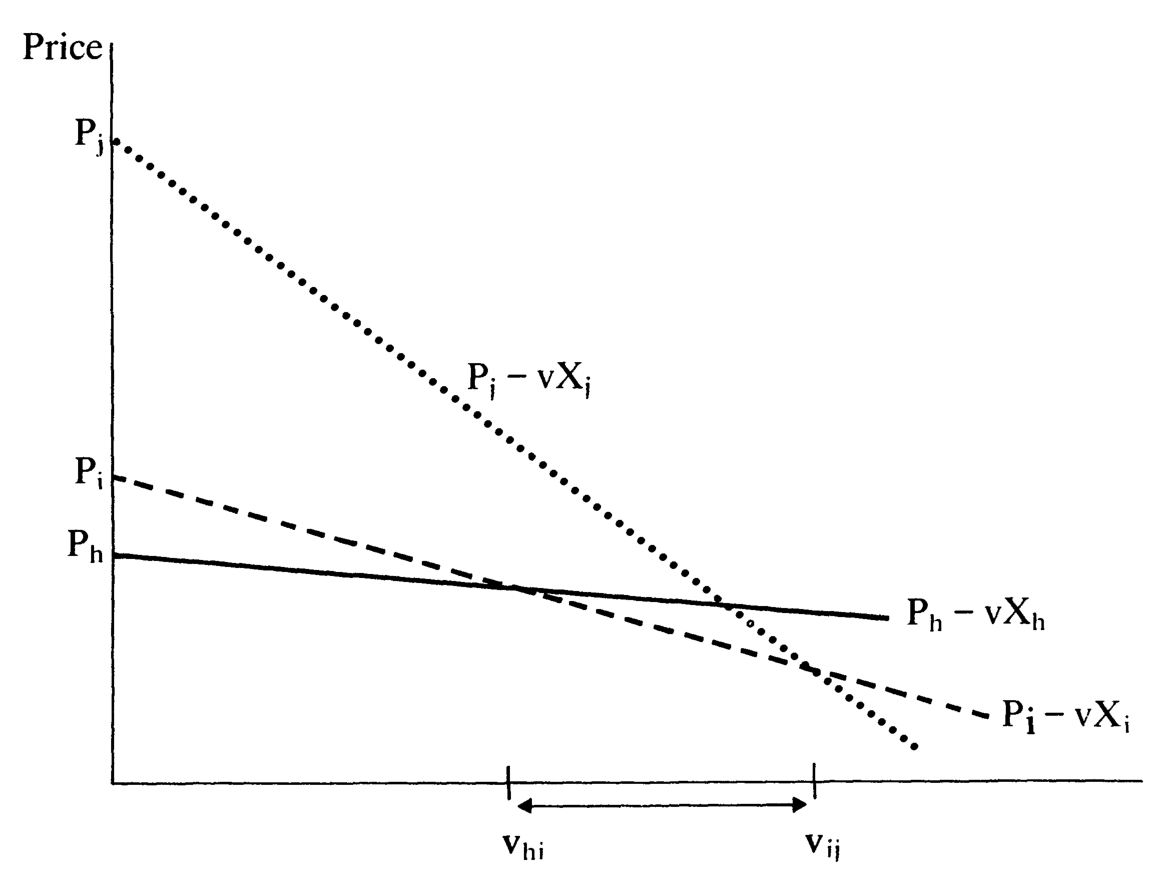
\includegraphics[width=\linewidth]{figures/ch06/bresnahan1987_fig1.png}
\caption{Total price lines in Bresnahan's form}
\end{subfigure}
\caption{Utility lines and cutoffs in the vertical model. (a) The utility $u_j(\nu) = \delta_j - \nu p_j$ of each
product is a line with intercept $\delta_j$ and slope $-p_j$, and the outside good is the horizontal axis.
The products are those of \cref{fig:06-frontier}. The bold upper envelope gives the chosen product, and
adjacent lines cross at the cutoffs $\bar\nu_3 < \bar\nu_2 < \bar\nu_1$, here $0.42$, $0.8$ and $1.6$. The
strip below the axis shows the product chosen on each interval of $\nu$. The dashed gray line is product
$b$, which never reaches the envelope. (b) The same construction in the form
$\frac{u_{ij}}{\nu_i} = v_i\delta_j - p_j$ used by \citet{Bresnahan1987}. A consumer with taste for quality
$v = \frac{1}{\nu}$ buys the product with the lowest total price $P - vX$, where Bresnahan writes $P$ for price and $X$ for
quality. Product $i$ is bought on the
marked interval $[v_{hi}, v_{ij}]$. Because $v$ is the reciprocal of $\nu$, the order of products along the
horizontal axis is reversed. Source: Bresnahan (1987), Figure 1.}
\label{fig:06-ulines}
\end{figure}

Without the frontier assumption, the same logic gives a single formula that holds for any qualities
\citep[eqs.~14--17]{BerryPakes2007}. Keep all products ordered by price, but let qualities be arbitrary.
Product $j$ beats product $k$ if and only if $\nu(p_j - p_k) < \delta_j - \delta_k$. For a cheaper product
$k < j$, dividing by $p_j - p_k > 0$ gives $\nu < \frac{\delta_j - \delta_k}{p_j - p_k}$. For a more expensive
product $k > j$, dividing by $p_j - p_k < 0$ reverses the inequality and gives
$\nu > \frac{\delta_k - \delta_j}{p_k - p_j}$. Product $j$ is chosen if and only if
$\underline\nu_j(\delta, p) < \nu < \bar\nu_j(\delta, p)$, where
\begin{equation}\label{eq:06-bp-cutoffs}
  \bar\nu_j(\delta, p) = \min_{k < j} \frac{\delta_j - \delta_k}{p_j - p_k}, \qquad
  \underline\nu_j(\delta, p) = \max_{k > j} \frac{\delta_k - \delta_j}{p_k - p_j},
\end{equation}
with the conventions $\bar\nu_0(\delta, p) = \infty$ and $\underline\nu_J(\delta, p) = 0$. The share of
product $j$ is
\begin{equation}\label{eq:06-bp-share}
  s_j = \big[F(\bar\nu_j(\delta, p)) - F(\underline\nu_j(\delta, p))\big]\,
        \indic\big\{\bar\nu_j(\delta, p) > \underline\nu_j(\delta, p)\big\}.
\end{equation}
\citet{BerryPakes2007} write these cutoffs as $\overline\Delta_j$ and $\underline\Delta_j$ and the price
sensitivity as $\alpha_i$.

\begin{remark}[General and adjacent cutoffs]\label{rem:06-general-cutoffs}
Formula \eqref{eq:06-bp-share} has three useful properties. First, for a product on the frontier,
$\bar\nu_j(\delta,p) = \bar\nu_j$ and $\underline\nu_j(\delta,p) = \bar\nu_{j+1}$, the adjacent cutoffs of
\eqref{eq:06-cutoff}. The slope of the chord from $j$ back to a cheaper frontier product $k$ is an average
of the edge slopes $\bar\nu_{k+1}, \dots, \bar\nu_j$. Each of these is at least $\bar\nu_j$, so the minimum is
attained at $k = j - 1$. Points below the frontier give chords at least as steep, so they do not change the minimum.
The same argument applies to the maximum. Second, the formula assigns a zero share to every product off the
frontier, so one expression serves for every parameter value. This matters in estimation, where a trial
parameter value can reorder qualities. Third, the vertical model predicts exact zero shares for some
parameter values, which models with an idiosyncratic shock never do. Since observed shares are positive,
the true parameters must place every product with positive sales on the frontier. Deleting the products
dominated outright is not enough to impose this. Product $b$ in \cref{fig:06-frontier} beats every cheaper
product in quality and still sells nothing.
\end{remark}

\subsection{Market shares}\label{sec:06-vshares}

Integrating the choice intervals over the taste distribution gives the demand system.

\begin{proposition}[Vertical market shares]\label{prop:06-vshares}
Under \cref{ass:06-vertical}, with all $J$ products on the frontier, the market shares are
\begin{equation}\label{eq:06-vshares}
  s_j = F(\bar\nu_j) - F(\bar\nu_{j+1}), \quad j = 1, \dots, J, \qquad
  s_0 = 1 - F(\bar\nu_1) = 1 - F\Big(\frac{\delta_1}{p_1}\Big),
\end{equation}
with $F(\bar\nu_{J+1}) = F(0) = 0$. Quantities are $q_j = M s_j$.
\end{proposition}

\begin{proof}
By \cref{prop:06-cutoffs}, $s_j = \Pr(\bar\nu_{j+1} < \nu_i < \bar\nu_j)$. Since $F$ is continuous, the end points
carry no mass, and $s_j = F(\bar\nu_j) - F(\bar\nu_{j+1})$. For the outside good, $s_0 = \Pr(\nu_i > \bar\nu_1) =
1 - F(\bar\nu_1)$. For the top product, $s_J = F(\bar\nu_J) - F(0) = F(\bar\nu_J)$. Summing over
$j = 0, \dots, J$ telescopes to one.
\end{proof}

Four features of \eqref{eq:06-vshares} recur below. Shares depend on qualities and prices only through
the $J$ cutoffs. The share of product $j$ depends only on its own price and the prices of its two
neighbors. The outside share depends only on the price and quality of the cheapest product. Zero shares
are possible, for any product off the frontier. \Cref{fig:06-nuaxis} draws the shares as areas under the
density.

\begin{figure}[htbp]
\centering
\begin{tikzpicture}
\begin{axis}[
  width=0.8\textwidth, height=5.6cm,
  xmin=0, xmax=3.05, ymin=0, ymax=1.12,
  axis lines=left,
  xlabel={price sensitivity $\nu$}, ylabel={$f(\nu)$},
  xtick={0.416667,0.8,1.6}, xticklabels={$\bar\nu_3$,$\bar\nu_2$,$\bar\nu_1$},
  ytick={0,0.5,1},
  clip=false,
]
  \addplot[name path=dens, thick, domain=0:3, samples=150] {exp(-x)};
  \path[name path=base] (axis cs:0,0) -- (axis cs:3,0);
  \addplot[fill=blue!45] fill between[of=dens and base, soft clip={domain=0:0.416667}];
  \addplot[fill=blue!28] fill between[of=dens and base, soft clip={domain=0.416667:0.8}];
  \addplot[fill=blue!14] fill between[of=dens and base, soft clip={domain=0.8:1.6}];
  \addplot[fill=gray!18] fill between[of=dens and base, soft clip={domain=1.6:3}];
  \draw[thin] (axis cs:0.416667,0) -- (axis cs:0.416667,{exp(-0.416667)});
  \draw[thin] (axis cs:0.8,0) -- (axis cs:0.8,{exp(-0.8)});
  \draw[thin] (axis cs:1.6,0) -- (axis cs:1.6,{exp(-1.6)});
  \node at (axis cs:0.2,0.33) {$s_3$};
  \node at (axis cs:0.61,0.25) {$s_2$};
  \node at (axis cs:1.2,0.15) {$s_1$};
  \node at (axis cs:2.05,0.06) {$s_0$};
  \node[anchor=west] at (axis cs:1.0,0.75) {$f(\nu) = e^{-\nu}$};
\end{axis}
\end{tikzpicture}
\caption{Market shares as areas under the taste density. The density is exponential with mean one, and the
cutoffs are those of \cref{fig:06-ulines}, $\bar\nu_3 = 0.42$, $\bar\nu_2 = 0.8$ and $\bar\nu_1 = 1.6$. The least
price-sensitive consumers buy the top product. The shares are $s_3 = 0.341$, $s_2 = 0.210$, $s_1 = 0.247$
and $s_0 = 0.202$.}
\label{fig:06-nuaxis}
\end{figure}

\begin{example}[Uniform tastes for quality]\label{ex:06-uniform}
\citet{Bresnahan1987} works with the form \eqref{eq:06-vertical-v} and assumes that the taste for quality
$v_i = \frac{1}{\nu_i}$ is uniform on $[0, \bar v]$ with density $\kappa$, so the market has $M = \kappa\bar v$
consumers.\footnote{Bresnahan writes quality as $x$, the taste density as $\delta$, and the upper bound
as $V_{\max}$. We write $\delta_j$, $\kappa$ and $\bar v$ to keep the notation of this chapter.} In
$v$-space the cutoff between $j-1$ and $j$ is the reciprocal of \eqref{eq:06-cutoff},
\begin{equation*}
  v_{j-1,j} = \frac{1}{\bar\nu_j} = \frac{p_j - p_{j-1}}{\delta_j - \delta_{j-1}},
\end{equation*}
and consumers with $v > v_{j-1,j}$ prefer $j$ \citep[eq.~4]{Bresnahan1987}. The implied CDF of
$\nu = \frac{1}{v}$ is
\begin{equation*}
  F(\nu) = \Pr\Big(v \ge \frac{1}{\nu}\Big) = 1 - \frac{1}{\bar v\,\nu}, \qquad \nu \ge \frac{1}{\bar v},
\end{equation*}
and zero below $\frac{1}{\bar v}$. Substituting into \eqref{eq:06-vshares},
\begin{equation*}
  s_j = \Big[1 - \frac{1}{\bar v\,\bar\nu_j}\Big] - \Big[1 - \frac{1}{\bar v\,\bar\nu_{j+1}}\Big]
      = \frac{1}{\bar v}\big(v_{j,j+1} - v_{j-1,j}\big),
\end{equation*}
so that $q_j = M s_j = \kappa\,(v_{j,j+1} - v_{j-1,j})$, or
\begin{equation}\label{eq:06-vuniform-demand}
  q_j = \kappa\Big[\frac{p_{j+1} - p_j}{\delta_{j+1} - \delta_j} - \frac{p_j - p_{j-1}}{\delta_j - \delta_{j-1}}\Big],
  \qquad
  q_J = \kappa\Big[\bar v - \frac{p_J - p_{J-1}}{\delta_J - \delta_{J-1}}\Big].
\end{equation}
These are equations (10) and (11) of \citet{Bresnahan1987}. Demand is linear in prices because the
cutoffs in $v$-space are linear in prices. The support of $\nu$ starts at $\frac{1}{\bar v}$ instead of
zero, so the top product sells only if $v_{J-1,J} < \bar v$. Bresnahan assumes that the consumer with the
highest taste, $\bar v$, always buys a car. In his application the alternative to a new car is a used
car of quality $\delta_{\mathrm u}$ and price $p_{\mathrm u}$, which replaces the origin as the point
$(p_0, \delta_0)$ (\cref{sec:06-vext}).
\end{example}

\subsection{Inverting market shares}\label{sec:06-vinversion}

Estimation requires the reverse map, from observed shares to qualities (\cref{sec:06-inversion-idea}). In
the vertical model the inverse exists, is unique, and has a closed form. Let
\begin{equation}\label{eq:06-cumshare}
  S_j = \sum_{k \ge j} s_k, \qquad j = 1, \dots, J,
\end{equation}
be the \emph{cumulative share from the top}, the share of consumers who buy product $j$ or a more
expensive product.

\begin{proposition}[Inversion]\label{prop:06-vinversion}
Under \cref{ass:06-vertical}, let the prices satisfy $0 < p_1 < \dots < p_J$ and let the observed shares
$s_j = \frac{q_j}{M}$ be positive for $j = 1, \dots, J$, with $s_0 = 1 - \sum_j s_j > 0$. There is exactly
one quality vector $\delta$ under which all $J$ products lie on the frontier and the predicted shares
\eqref{eq:06-vshares} equal the observed shares. It is given by
\begin{align}
  \bar\nu_j &= F^{-1}(S_j), \label{eq:06-vinv-cut}\\
  \delta_j &= \delta_{j-1} + (p_j - p_{j-1})\,F^{-1}(S_j), \qquad \delta_0 = 0, \label{eq:06-vinv-rec}\\
  \delta_j &= \sum_{m=1}^{j} (p_m - p_{m-1})\, F^{-1}\Big(\sum_{k \ge m} s_k\Big). \label{eq:06-vinv-sum}
\end{align}
\end{proposition}

\begin{proof}
The first step sums shares from the top. Under \eqref{eq:06-vshares},
\begin{equation*}
  S_j = \sum_{k=j}^{J} \big[F(\bar\nu_k) - F(\bar\nu_{k+1})\big] = F(\bar\nu_j) - F(\bar\nu_{J+1}) = F(\bar\nu_j).
\end{equation*}
The second step proves uniqueness. Because $F$ is continuous and strictly increasing on $(0,\infty)$, its
inverse $F^{-1}$ is well defined on $(0,1)$. Each $S_j$ lies in $(0,1)$, since $s_J > 0$ and
$1 - S_1 = s_0 > 0$. Hence $\bar\nu_j = F^{-1}(S_j)$ is the only cutoff consistent with the data. The
definition \eqref{eq:06-cutoff} gives $\delta_j - \delta_{j-1} = (p_j - p_{j-1})\bar\nu_j$, which is
\eqref{eq:06-vinv-rec}. Starting from $\delta_0 = 0$ and iterating gives \eqref{eq:06-vinv-sum}, so every
quality is pinned down.

The third step proves existence. Define $\delta$ by \eqref{eq:06-vinv-sum}. All shares are positive, so
$S_1 > S_2 > \dots > S_J > 0$. Because $F^{-1}$ is strictly increasing, $\bar\nu_1 > \bar\nu_2 > \dots > \bar\nu_J
> 0$. Qualities then increase with price and the cutoffs decrease, so by \cref{prop:06-frontier} every
product lies on the frontier. \Cref{prop:06-vshares} gives predicted shares
$F(\bar\nu_j) - F(\bar\nu_{j+1}) = S_j - S_{j+1} = s_j$.
\end{proof}

Several consequences follow. The price ordering determines the quality ordering, so the data reveal the
ranking of products without any parameter. Every vector of positive shares is rationalized by some quality
vector, whatever the increasing distribution $F$. A single market's prices and shares therefore never
reject the vertical model. Its testable content comes from restrictions across products and markets, such
as $\delta_{jt} = x_{jt}\beta + \xi_{jt}$, and from the supply side.

The result is an instance of the general invertibility theory of \citet{BerryGandhiHaile2013}. On the set
of qualities at which every product sells, raising $\delta_j$ raises $\bar\nu_j$ and lowers $\bar\nu_{j+1}$.
It therefore raises $s_j$, lowers $s_{j-1}$ and $s_{j+1}$ (or $s_0$ when $j = 1$), and leaves every other
share unchanged. Inside goods are weak substitutes in this sense. The chain $0, 1, \dots, J$ of strict
substitution between neighbors connects every inside good to the outside good. These are the ``connected
substitutes'' conditions under which \citet{BerryGandhiHaile2013} prove that demand is invertible. The
proof above exploits the special structure and also delivers the inverse in closed form.

Market size enters through every share. Holding unit sales fixed, a larger $M$ lowers every cumulative
share $S_j$, which lowers every cutoff and every quality. A market with more nonbuyers is rationalized by
products that are worse relative to the outside good. The choice of $M$ is an assumption, and it
matters for the level of the recovered qualities.

\begin{example}[Exponential tastes]\label{ex:06-exponential}
Let $F(\nu) = 1 - e^{-\lambda\nu}$ with $\lambda > 0$, so that $\E[\nu_i] = \frac{1}{\lambda}$. Solving
$u = 1 - e^{-\lambda\nu}$ for $\nu$ gives
\begin{equation*}
  F^{-1}(u) = -\frac{1}{\lambda}\ln(1 - u).
\end{equation*}
Substituting into \eqref{eq:06-vinv-sum},
\begin{equation}\label{eq:06-vexp-delta}
  \delta_j = -\frac{1}{\lambda}\sum_{m=1}^{j}(p_m - p_{m-1})\ln(1 - S_m),
  \qquad 1 - S_m = s_0 + \sum_{l < m} s_l ,
\end{equation}
where $1 - S_m$ is the share of consumers who buy the outside good or a product cheaper than $m$. Now let
there be markets $t = 1, \dots, T$, and let $(m)$ denote the $m$-th cheapest product of market $t$. For the
product $j$ that occupies position $k$ in market $t$, define the observable
\begin{equation}\label{eq:06-vexp-y}
  y_{jt} \equiv -\sum_{m=1}^{k}\big(p_{(m)t} - p_{(m-1)t}\big)\ln(1 - S_{mt}),
\end{equation}
which uses prices and shares only. By \eqref{eq:06-vexp-delta}, $y_{jt} = \lambda\delta_{jt}$. Substituting
$\delta_{jt} = x_{jt}\beta + \xi_{jt}$ gives the estimable equation
\begin{equation}\label{eq:06-vexp-reg}
  y_{jt} = x_{jt}(\lambda\beta) + \lambda\xi_{jt} .
\end{equation}
\end{example}

\begin{proposition}[Scale of tastes]\label{prop:06-vscale}
In \cref{ex:06-exponential}, $\lambda$ is not identified. For every $c > 0$ the parameters
$(\lambda, \beta, \xi)$ and $(\frac{\lambda}{c}, c\beta, c\xi)$ imply the same choice for every consumer and
hence the same shares. More generally, for any $F$, the pairs $(F(\cdot), \delta)$ and
$(F(\frac{\cdot}{c}), c\delta)$ are observationally equivalent.
\end{proposition}

\begin{proof}
Let $\nu$ have CDF $F$ and define $\nu' = c\nu$. Then $\Pr(\nu' \le x) = \Pr(\nu \le \frac{x}{c}) = F(\frac{x}{c})$.
A consumer of type $\nu$ facing qualities $\delta$ compares $\delta_j - \nu p_j$ across products. Multiplying
by $c > 0$ gives
\begin{equation*}
  c\delta_j - (c\nu)p_j = c\delta_j - \nu' p_j ,
\end{equation*}
which ranks products in the same order. So a consumer of type $\nu'$ facing qualities $c\delta$ makes the
same choice as a consumer of type $\nu$ facing $\delta$. Integrating over types, the shares under
$(F(\frac{\cdot}{c}), c\delta)$ equal those under $(F, \delta)$. For the exponential distribution,
$F(\frac{x}{c}) = 1 - e^{-\frac{\lambda}{c}x}$ is exponential with parameter $\frac{\lambda}{c}$, and
$c\delta_j = x_j(c\beta) + c\xi_j$.
\end{proof}

The economic content is that choices reveal quality only in units of willingness to pay. Doubling every
quality and doubling every consumer's price sensitivity describes the same consumers making the same
choices. This is the scale normalization of \cref{sec:06-normalization} in the vertical model. We set
$\lambda = 1$, so that $\E[\nu_i] = 1$. A consumer with the mean price sensitivity then values one unit of
quality at one dollar, and \eqref{eq:06-vexp-reg} becomes $y_{jt} = x_{jt}\beta + \xi_{jt}$.

With $\lambda = 1$ the demand parameters are identified under two conditions. The first is the moment
condition $\E[x_{jt}^\top\xi_{jt}] = 0$, and the second is full rank of $\E[x_{jt}^\top x_{jt}]$. Then
$\beta = \E[x_{jt}^\top x_{jt}]^{-1}\E[x_{jt}^\top y_{jt}]$, and the OLS regression of $y_{jt}$ on $x_{jt}$ is
consistent. Price is not a regressor. It enters only the construction of $y_{jt}$, an exact function of
observed prices and shares. Firms that observe $\xi_{jt}$ set higher prices for better products, so
$p_{jt}$ and $\xi_{jt}$ are correlated. This correlation does not bias the regression, because the vertical
model has no price coefficient left to estimate. The normalized distribution $F$ plays the role of the
price coefficient. It states how many consumers have each price sensitivity, and nothing about it remains
unknown. Standard errors should be clustered by market. The values $y_{jt}$ of products in the same market
are built from the same cumulative shares. Any sampling error in observed shares, or any misspecification of $F$,
therefore enters the errors of all products in a market and accumulates along the price ladder.

The same feature is the model's main weakness. With $F$ fully specified, every substitution pattern is
determined by functional form and by the observed prices and shares (\cref{prop:06-vmarkup-data} below).
Exogenous variation in prices is never used to learn how demand responds to prices. Two further cautions
apply. The moment condition fails if firms choose characteristics with knowledge of $\xi_{jt}$
(\cref{sec:06-charspace}). If $F$ is misspecified, $y_{jt}$ differs from $\delta_{jt}$ by a function of
prices and shares, and the regression error inherits that function.

\begin{remark}[Shape parameters and instruments]\label{rem:06-vshape}
Suppose that after the scale normalization $F$ still has an unknown shape parameter. An example is
$\ln\nu_i \sim N(0, \sigma^2)$, whose median is fixed at one. With $\Phi$ the standard normal CDF,
$F_\sigma^{-1}(u) = \exp(\sigma\Phi^{-1}(u))$, and the inversion gives
\begin{equation*}
  \delta_{jt}(\sigma) = \sum_{m=1}^{k}\big(p_{(m)t} - p_{(m-1)t}\big)\exp\big(\sigma\,\Phi^{-1}(S_{mt})\big).
\end{equation*}
For any trial value of $\sigma$, OLS of $\delta_{jt}(\sigma)$ on $x_{jt}$ produces residuals orthogonal to
$x_{jt}$. The $K$ moments $\E[x_{jt}^\top\xi_{jt}] = 0$ therefore cannot determine the $K + 1$ parameters
$(\beta, \sigma)$. Identification of $\sigma$ requires at least one excluded instrument $z_{jt}$. This is a variable
uncorrelated with $\xi_{jt}$ that moves prices or shares, such as a cost shifter or a characteristic of
rival products. Stack the instruments in $Z_{jt} = (x_{jt}, z_{jt})$ and define
$\xi_{jt}(\sigma, \beta) = \delta_{jt}(\sigma) - x_{jt}\beta$. The GMM estimator uses
$\E[Z_{jt}^\top\xi_{jt}(\sigma,\beta)] = 0$. For fixed $\sigma$ the estimate of $\beta$ is the linear IV
estimator
\begin{equation*}
  \hat\beta(\sigma) = (X^\top Z W Z^\top X)^{-1} X^\top Z W Z^\top\delta(\sigma),
\end{equation*}
where $X$, $Z$ and $\delta(\sigma)$ stack the observations and $W$ is a weighting matrix. Concentrating out
$\beta$ leaves a search over $\sigma$ alone,
\begin{equation*}
  \hat\sigma = \argmin_{\sigma}\; g_N(\sigma)^\top W g_N(\sigma), \qquad
  g_N(\sigma) = \frac{1}{N}\sum_{j,t} Z_{jt}^\top\big(\delta_{jt}(\sigma) - x_{jt}\hat\beta(\sigma)\big).
\end{equation*}
This is the structure of the estimator for the nonlinear parameters $\theta_2$ in \cref{ch:blp}. Price
endogeneity now matters. Prices enter $\delta_{jt}(\sigma)$ in a way that depends on $\sigma$, so the
instruments must move prices independently of $\xi_{jt}$. Standard errors are again clustered by market.
\end{remark}

The uniform model of \cref{ex:06-uniform} inverts in the same way. Summing \eqref{eq:06-vuniform-demand} from
the top gives $\sum_{k \ge j} q_k = \kappa(\bar v - v_{j-1,j})$. Dividing by $M = \kappa\bar v$ gives
$v_{j-1,j} = \bar v(1 - S_j)$, so
\begin{equation*}
  \delta_j - \delta_{j-1} = \frac{p_j - p_{j-1}}{\bar v(1 - S_j)} .
\end{equation*}
Given the market size, $\bar v$ only sets the units of quality, in line with \cref{prop:06-vscale}.

\subsection{Substitution patterns}\label{sec:06-vsubst}

We now hold qualities fixed and differentiate shares with respect to prices. Each price enters only the
two cutoffs that involve its product. Differentiating \eqref{eq:06-cutoff},
\begin{align*}
  \frac{\partial\bar\nu_j}{\partial p_j} &= -\frac{\delta_j - \delta_{j-1}}{(p_j - p_{j-1})^2} = -\frac{\bar\nu_j}{p_j - p_{j-1}},
  &
  \frac{\partial\bar\nu_j}{\partial p_{j-1}} &= \frac{\delta_j - \delta_{j-1}}{(p_j - p_{j-1})^2} = \frac{\bar\nu_j}{p_j - p_{j-1}},
\end{align*}
and, shifting the index,
\begin{equation*}
  \frac{\partial\bar\nu_{j+1}}{\partial p_j} = \frac{\bar\nu_{j+1}}{p_{j+1} - p_j},
  \qquad
  \frac{\partial\bar\nu_{j+1}}{\partial p_{j+1}} = -\frac{\bar\nu_{j+1}}{p_{j+1} - p_j}.
\end{equation*}
A higher own price lowers the upper cutoff of $j$ and raises its lower cutoff, so the interval of buyers
shrinks from both ends. It is convenient to define
\begin{equation}\label{eq:06-gj}
  g_j = f(\bar\nu_j)\,\frac{\bar\nu_j}{p_j - p_{j-1}} > 0, \quad j = 1, \dots, J, \qquad g_{J+1} = 0 .
\end{equation}
The number $g_j$ is the density of consumers at the boundary between $j - 1$ and $j$, times the speed at
which that boundary moves when either price changes.

\begin{proposition}[Price derivatives]\label{prop:06-vderiv}
Under \cref{ass:06-vertical}, with all products on the frontier and qualities held fixed,
\begin{align}
  \frac{\partial s_j}{\partial p_j} &= -g_j - g_{j+1}
     = -\frac{f(\bar\nu_j)\bar\nu_j}{p_j - p_{j-1}} - \frac{f(\bar\nu_{j+1})\bar\nu_{j+1}}{p_{j+1} - p_j}, \label{eq:06-vown}\\
  \frac{\partial s_j}{\partial p_{j-1}} &= g_j, \qquad \frac{\partial s_j}{\partial p_{j+1}} = g_{j+1}, \qquad
  \frac{\partial s_j}{\partial p_k} = 0 \ \text{ for } |k - j| \ge 2, \label{eq:06-vcross}\\
  \frac{\partial s_0}{\partial p_1} &= g_1, \qquad \frac{\partial s_0}{\partial p_k} = 0 \ \text{ for } k \ge 2.
  \label{eq:06-voutside}
\end{align}
The second term of \eqref{eq:06-vown} is absent for the top product. The $J \times J$ Jacobian $\Delta^s$ with
$\Delta^s_{jk} = \frac{\partial s_j}{\partial p_k}$ is tridiagonal and symmetric, with
$\Delta^s_{j,j+1} = \Delta^s_{j+1,j} = g_{j+1}$. Each column of the $(J+1) \times J$ matrix that adds the outside-good
row sums to zero.
\end{proposition}

\begin{proof}
Write $s_j = F(\bar\nu_j) - F(\bar\nu_{j+1})$. The price $p_j$ enters $\bar\nu_j$ and $\bar\nu_{j+1}$ only, so by the
chain rule
\begin{equation*}
  \frac{\partial s_j}{\partial p_j} = f(\bar\nu_j)\frac{\partial\bar\nu_j}{\partial p_j} - f(\bar\nu_{j+1})\frac{\partial\bar\nu_{j+1}}{\partial p_j}
  = -f(\bar\nu_j)\frac{\bar\nu_j}{p_j - p_{j-1}} - f(\bar\nu_{j+1})\frac{\bar\nu_{j+1}}{p_{j+1} - p_j}.
\end{equation*}
The price $p_{j-1}$ enters $s_j$ only through $\bar\nu_j$, so $\frac{\partial s_j}{\partial p_{j-1}} =
f(\bar\nu_j)\frac{\bar\nu_j}{p_j - p_{j-1}} = g_j$. The price $p_{j+1}$ enters $s_j$ only through $\bar\nu_{j+1}$,
so
\begin{equation*}
  \frac{\partial s_j}{\partial p_{j+1}} = -f(\bar\nu_{j+1})\frac{\partial\bar\nu_{j+1}}{\partial p_{j+1}}
  = f(\bar\nu_{j+1})\frac{\bar\nu_{j+1}}{p_{j+1} - p_j} = g_{j+1}.
\end{equation*}
No other price enters $s_j$. For the outside good, $s_0 = 1 - F(\bar\nu_1)$ with $\bar\nu_1 = \frac{\delta_1}{p_1}$,
so $\frac{\partial s_0}{\partial p_1} = f(\bar\nu_1)\frac{\bar\nu_1}{p_1} = g_1$. Symmetry follows by comparing
$\Delta^s_{j,j+1} = g_{j+1}$ with $\Delta^s_{j+1,j} = \frac{\partial s_{j+1}}{\partial p_j} = g_{j+1}$, the second identity
in \eqref{eq:06-vcross} applied to product $j+1$. Column $k$ has the entries $g_k$ in row $k - 1$ (the outside
row when $k = 1$), $-g_k - g_{k+1}$ in row $k$, and $g_{k+1}$ in row $k + 1$. They sum to zero.
\end{proof}

Symmetry has a simple reading. The number $g_{j+1}$ measures the consumers at the boundary between $j$
and $j + 1$. A small rise in $p_j$ moves these marginal consumers from $j$ to $j + 1$, and an equal rise in
$p_{j+1}$ moves the same consumers back. The flow across a shared boundary is the same in both directions.
Symmetry also follows from the envelope argument behind \cref{thm:06-wdz}. Dividing utility by $\nu_i$ gives
$\frac{u_{ij}}{\nu_i} = \frac{\delta_j}{\nu_i} - p_j$, which is quasi-linear in money for each consumer.
Aggregate consumer surplus $CS(p) = M\,\E\big[\max_j(\frac{\delta_j}{\nu_i} - p_j)\big]$ therefore satisfies
$\frac{\partial CS}{\partial p_j} = -q_j$, and the symmetry of its second derivatives gives
$\frac{\partial q_j}{\partial p_k} = \frac{\partial q_k}{\partial p_j}$. The zero column sums say that a price
change only reallocates the $M$ consumers among the alternatives.

The structure of $\Delta^s$ has further consequences used in \cref{sec:06-vpricing}. In row $j$ with
$2 \le j \le J$, the off-diagonal entries $g_j$ and $g_{j+1}$ sum to $|\Delta^s_{jj}|$. In the first row,
$|\Delta^s_{11}| = g_1 + g_2$ exceeds the single off-diagonal entry $g_2$, because product 1 also loses consumers
to the outside good. So $\Delta^s$ is weakly diagonally dominant, strictly so in the first row. Because $\Delta^s$ is
tridiagonal with nonzero off-diagonal entries, it is also irreducible. An irreducible matrix that is weakly
diagonally dominant with at least one strictly dominant row is nonsingular \citep[ch.~6]{BermanPlemmons1994}.
\Cref{lem:06-mmatrix} in \cref{sec:06-bres-equilibrium} states and proves this fact in the form we need.

The \emph{diversion ratio} from $j$ to $k$ is the fraction of the consumers lost by $j$ after a price
increase who switch to $k$ (\cref{ch:diffprod}). We write it $D_{jk} = -\frac{\Delta^s_{kj}}{\Delta^s_{jj}}$. Here
\begin{equation*}
  D_{j,j-1} = \frac{g_j}{g_j + g_{j+1}}, \qquad
  D_{j,j+1} = \frac{g_{j+1}}{g_j + g_{j+1}},
\end{equation*}
and all other diversion ratios are zero. Every consumer who leaves $j$ goes to a price neighbor, with the
outside good counting as the lower neighbor of product 1.

We write the elasticity of the share of $j$ with respect to the price of $k$ as
$\varepsilon_{jk} = \frac{\partial s_j}{\partial p_k}\frac{p_k}{s_j}$. The diagonal entries are negative, and the
own-price elasticity in the positive convention of the book is $\varepsilon_j = -\varepsilon_{jj} =
\frac{(g_j + g_{j+1})p_j}{s_j}$. The outside good has the single nonzero elasticity
$\varepsilon_{01} = \frac{g_1 p_1}{s_0}$.

Closeness in price means closeness in substitution. Holding a cutoff fixed, the cross derivative
$g_{j+1} = f(\bar\nu_{j+1})\frac{\bar\nu_{j+1}}{p_{j+1} - p_j}$ grows without bound as $p_{j+1} - p_j \to 0$, and the
own derivatives of both products grow with it. In the data the cutoff is pinned down by shares through
$\bar\nu_{j+1} = F^{-1}(S_{j+1})$. Two products that sell at nearly the same price are therefore read as
near-perfect substitutes, whatever the products are. With uniform tastes the derivatives are constant.
Using $f(\nu) = \frac{1}{\bar v\nu^2}$ from \cref{ex:06-uniform},
\begin{equation*}
  M g_j = \kappa\bar v\cdot\frac{1}{\bar v\,\bar\nu_j^2}\cdot\frac{\bar\nu_j}{p_j - p_{j-1}}
        = \frac{\kappa}{\bar\nu_j(p_j - p_{j-1})} = \frac{\kappa}{\delta_j - \delta_{j-1}} .
\end{equation*}
Hence $\frac{\partial q_j}{\partial p_j} = -\kappa\big(\frac{1}{\delta_j - \delta_{j-1}} + \frac{1}{\delta_{j+1} - \delta_j}\big)$
and $\frac{\partial q_{j\pm1}}{\partial p_j} = \frac{\kappa}{|\delta_{j\pm1} - \delta_j|}$. Demand is linear, and the
quality gap measures how close two products are. In Bresnahan's words, the products are perfect
substitutes ``in the limit as $x_i$ goes to $x_h$,'' where $x$ is his notation for quality
\citep[p.~462]{Bresnahan1987}.

Is this a reasonable model of substitution? The restriction that only price neighbors substitute is
strong. A price cut on a mid-size sedan has no effect on a model two steps away on the price ladder,
however similar the two cars are physically. Conversely, a minivan and a sports car at the same price are
treated as close substitutes because they are neighbors on the ladder. The restriction is natural where
quality is essentially one-dimensional, as with airline cabins or storage tiers. It is also the source of
the power of the conduct test in \cref{sec:06-bresnahan}. Where products differ along several dimensions,
it can mislead badly.

A simulated illustration shows how badly (\cref{app:problems}). Market data are generated by a random
coefficients logit model in 100 markets, each offering between four and nine of ten products. The vertical
model with exponential tastes and $\lambda = 1$ is then fitted to these data. In one market the fitted own-price
elasticities $\varepsilon_{jj}$ range from $-358.4$ to $-16.8$, while the true $\varepsilon_{jj}$ range from $-3.85$
to $-2.57$. The largest
elasticities belong to products whose price neighbor sells at almost the same price. The two products with the
largest elasticities in that market are price neighbors whose prices differ by only 0.019. Across all markets, the median gap between
adjacent prices is 0.057, and 58 of the 554 gaps are below 0.01. The vertical model can explain why
consumers split across products with similar prices only by placing those products almost on top of each
other in quality. Under multi-product Nash pricing it then implies a mean markup of 0.048, against a true
mean markup of 0.386.

\subsection{Pricing and recovering marginal costs}\label{sec:06-vpricing}

Firms indexed by $f$ own disjoint sets of products $\mathcal J_f$ and produce at constant marginal costs
$mc_j$. Firm
$f$ chooses the prices of its products to maximize $M\sum_{k \in \mathcal J_f}(p_k - mc_k)s_k(p)$. The
first-order condition for $p_j$, $j \in \mathcal J_f$, is
\begin{equation*}
  s_j + \sum_{k \in \mathcal J_f}(p_k - mc_k)\frac{\partial s_k}{\partial p_j} = 0 .
\end{equation*}
With the ownership matrix $\Omega$ ($\Omega_{jk} = 1$ if $j$ and $k$ have the same owner) and $\odot$ the
element-wise product, the conditions stack into
\begin{equation}\label{eq:06-vfoc-matrix}
  s + (\Omega \odot \Delta^{s\top})(p - mc) = 0
  \qquad\Longrightarrow\qquad
  mc = p + (\Omega \odot \Delta^{s\top})^{-1}s ,
\end{equation}
the multi-product markup formula of \cref{ch:diffprod}. By \cref{prop:06-vderiv}, the condition for product
$j$ involves only its neighbors. Writing $m_j = p_j - mc_j$ for the markup,
\begin{equation}\label{eq:06-vfoc}
  s_j - (g_j + g_{j+1})\,m_j + \Omega_{j,j+1}\,g_{j+1}\,m_{j+1} + \Omega_{j,j-1}\,g_j\,m_{j-1} = 0,
\end{equation}
with $\Omega_{1,0} = 0$ because the outside good earns no markup. A single-product firm sets
$m_j = \frac{s_j}{g_j + g_{j+1}}$, which is the inverse elasticity rule $\frac{m_j}{p_j} = \frac{1}{\varepsilon_j}$.
Equation \eqref{eq:06-vfoc} is the general-$F$ version of the conduct equation that \citet{Bresnahan1987}
estimates (\cref{sec:06-bresnahan}).

\begin{corollary}[Only neighbors' ownership matters]\label{cor:06-neighbors}
Under the conditions of \cref{prop:06-vderiv}, the matrix $\Omega \odot \Delta^{s\top}$ is block diagonal. Each
block corresponds to a maximal run of consecutive products with the same owner. Two ownership structures
that agree on which adjacent pairs share an owner imply the same first-order conditions, and hence the
same markups and implied marginal costs. Moreover, $\Omega \odot \Delta^{s\top}$ is nonsingular, and the markups
$m = -(\Omega \odot \Delta^{s\top})^{-1}s$ are positive.
\end{corollary}

\begin{proof}
Because $\Delta^{s\top}$ is tridiagonal, $(\Omega \odot \Delta^{s\top})_{jk} = \Omega_{jk}\Delta^s_{kj}$ vanishes unless $|j - k| \le 1$.
For $|j - k| = 1$ it equals $g_{\max\{j,k\}}$ if the two products share an owner and zero otherwise. So the
matrix depends on $\Omega$ only through the entries $\Omega_{j,j+1}$, and it breaks into blocks at every
adjacent pair with different owners. Within a block that starts at product $a$, the first row has diagonal
entry $-(g_a + g_{a+1})$ and off-diagonal entry $g_{a+1}$, so it is strictly diagonally dominant by
$g_a > 0$. The other rows are weakly dominant, as in the discussion after \cref{prop:06-vderiv}. Each block
is tridiagonal with nonzero off-diagonal entries, hence irreducible. The negative of each block therefore
has a positive diagonal, nonpositive off-diagonal entries, nonnegative row sums and a strictly positive
first row sum. By \cref{lem:06-mmatrix}(a) it is a nonsingular M-matrix whose inverse has positive entries. Since $s > 0$, the markups $m = \big(-(\Omega \odot \Delta^{s\top})\big)^{-1}s$ are
positive.
\end{proof}

The corollary is a sharp prediction. A firm that owns products 1 and 3 but not product 2 prices exactly
as two independent firms would. Joint ownership raises markups only when it links products that
compete for the same marginal consumers.

The vertical model has a second, more surprising property. When $F$ is known up to scale, the markups
require no demand estimate at all.

\begin{proposition}[Markups from prices and shares]\label{prop:06-vmarkup-data}
Under \cref{ass:06-vertical}, suppose $F(\nu) = F_1(\lambda\nu)$ for a known CDF $F_1$ with density $f_1$
and an unknown scale $\lambda > 0$. Then the Jacobian $\Delta^s$, the markups $-(\Omega \odot \Delta^{s\top})^{-1}s$ and the
implied marginal costs depend only on observed prices and shares. They depend on no demand parameter,
including $\lambda$ and $\beta$. With exponential tastes,
\begin{equation}\label{eq:06-vexp-g}
  \bar\nu_j = -\frac{1}{\lambda}\ln(1 - S_j), \qquad f(\bar\nu_j) = \lambda(1 - S_j), \qquad
  g_j = \frac{-(1 - S_j)\ln(1 - S_j)}{p_j - p_{j-1}} .
\end{equation}
\end{proposition}

\begin{proof}
By \cref{prop:06-vinversion}, $\bar\nu_j = F^{-1}(S_j) = \frac{1}{\lambda}F_1^{-1}(S_j)$. The density is
$f(\nu) = \lambda f_1(\lambda\nu)$. Hence
\begin{equation*}
  f(\bar\nu_j)\,\bar\nu_j = \lambda f_1\big(F_1^{-1}(S_j)\big)\cdot\frac{1}{\lambda}F_1^{-1}(S_j)
  = f_1\big(F_1^{-1}(S_j)\big)\,F_1^{-1}(S_j),
\end{equation*}
and $g_j = \frac{f_1(F_1^{-1}(S_j))F_1^{-1}(S_j)}{p_j - p_{j-1}}$ depends on prices and shares only.
\Cref{prop:06-vderiv} builds $\Delta^s$ from the $g_j$, and \eqref{eq:06-vfoc-matrix} builds the markups and
marginal costs from $\Delta^s$, $s$ and $p$. For the exponential case, $F_1(x) = 1 - e^{-x}$, so
$F_1^{-1}(u) = -\ln(1 - u)$ and $f_1(F_1^{-1}(u)) = e^{\ln(1-u)} = 1 - u$.
\end{proof}

The scale drops out for a reason. Markups are measured in dollars, while the scale normalization concerns
the units of utility, so no choice of units can change them. The proposition has two practical
consequences. First, the supply side can be estimated without any demand estimate. The implied marginal
cost of each product is a known function of the data. Second, demand and supply share no parameter. When
the demand error $\xi_{jt}$ and the cost error $\omega_{jt}$ are independent, estimating the two equations
separately loses no efficiency. The flip side is the caution raised in \cref{sec:06-vinversion}. The
model reads market power off the spacing of prices and the cumulative shares, never off exogenous price
variation.

The supply equations take two forms, one per conduct assumption. Under marginal-cost pricing,
\begin{equation}\label{eq:06-vsupply-mc}
  p_{jt} = x_{jt}\gamma_1 + \gamma_2 z_{jt} + \omega_{jt} .
\end{equation}
Under multi-product Nash pricing,
\begin{equation}\label{eq:06-vsupply-nash}
  p_{jt} + \big[(\Omega_t \odot \Delta_t^{s\top})^{-1}s_t\big]_j = x_{jt}\gamma_1 + \gamma_2 z_{jt} + \omega_{jt} .
\end{equation}
Here $z_{jt}$ is a cost shifter excluded from demand, and $\gamma_1$ and $\gamma_2$ are cost coefficients,
unrelated to Euler's constant $\gamma_E$. Under either assumption the left side is data, so OLS under
$\E[\omega_{jt} \mid x_{jt}, z_{jt}] = 0$ estimates the cost parameters. The conduct assumption determines how
large the markup is, and so how much of the price variation across products is attributed to cost.
Comparing the two specifications is the logic of the conduct test in \cref{sec:06-bresnahan}.

\begin{remark}[Existence of a price equilibrium]\label{rem:06-vexist}
\citet[footnote~6]{Bresnahan1987} observes that a price equilibrium always exists in quality models of
this kind, while it can fail in location models. With uniform tastes, consider product $j$ as its own price
falls. Its interval of buyers widens, and at some price the next product $j + 1$ is dominated out of the
market. Demand for $j$ stays continuous at that price, because the interval of $j + 1$ shrinks continuously
to zero. The slope of demand changes from $-\kappa\big(\frac{1}{\delta_{j+1} - \delta_j} + \frac{1}{\delta_j - \delta_{j-1}}\big)$
to $-\kappa\big(\frac{1}{\delta_{j+2} - \delta_j} + \frac{1}{\delta_j - \delta_{j-1}}\big)$. The second is smaller in
absolute value, because $\delta_{j+2} - \delta_j > \delta_{j+1} - \delta_j$. So demand is flatter below the kink
than above it, and the derivative $\frac{\partial q_j}{\partial p_j}$ falls as $p_j$ rises. Demand is concave in own
price across the kink, and the same holds where the lower neighbor drops out. Profit $(p_j - mc_j)q_j$ is
then concave in $p_j$ on the range of prices at which $j$ sells with a positive markup, and it is zero beyond
that range. Profit is therefore quasi-concave, and standard fixed-point arguments give an equilibrium. In the Hotelling model with linear costs, demand jumps when a firm captures the rival's
location, and existence can fail (\cref{sec:06-hotelling}). \citet[Theorem~2]{CaplinNalebuff1991} cover general taste
densities with single-product firms. Utility must be linear in the taste parameter, as in \eqref{eq:06-vertical-v}
with type $v_i$. The density of $v_i$ must be $\rho$-concave with $\rho = -\frac{1}{2}$, the case $n = 1$ of their
assumption A2. This means that $\frac{1}{\sqrt{f}}$ is convex, a condition that every log-concave density meets
(\cref{sec:06-branches} and \cref{ch:diffprod}).
\end{remark}

\begin{example}[A worked example]\label{ex:06-vnumeric}
Three products and an outside good face exponential tastes with $\lambda = 1$. Observed prices are
$p = (1.0, 1.5, 2.5)$ and observed shares are $s = (0.20, 0.15, 0.10)$, so $s_0 = 0.55$. \Cref{tab:06-vnumeric}
reports every step, computed to more digits than shown.

The first step inverts the shares. Cumulative shares are $S = (0.45, 0.25, 0.10)$. By \eqref{eq:06-vexp-g},
the cutoffs are $\bar\nu_1 = -\ln 0.55 = 0.598$, $\bar\nu_2 = -\ln 0.75 = 0.288$ and $\bar\nu_3 = -\ln 0.90 = 0.105$.
They decrease, as \cref{prop:06-vinversion} guarantees, so all three products are on the frontier. The
recursion \eqref{eq:06-vinv-rec} gives
\begin{align*}
  \delta_1 &= 1.0 \times 0.598 = 0.598,\\
  \delta_2 &= 0.598 + 0.5 \times 0.288 = 0.742,\\
  \delta_3 &= 0.742 + 1.0 \times 0.105 = 0.847 .
\end{align*}
Recomputing the shares at these qualities with \eqref{eq:06-bp-share} returns the observed shares
exactly. Simulating two million consumers returns them up to simulation error.

The second step computes substitution. The densities at the cutoffs are $f(\bar\nu_j) = 1 - S_j = (0.55, 0.75,
0.90)$. Formula \eqref{eq:06-gj} gives $g_1 = \frac{0.55 \times 0.598}{1.0} = 0.329$, $g_2 = \frac{0.75 \times 0.288}{0.5}
= 0.432$ and $g_3 = \frac{0.90 \times 0.105}{1.0} = 0.095$. These fill the Jacobian through
\cref{prop:06-vderiv}. Product 2 has the most elastic demand, $\varepsilon_2 = 5.26$. It sits between two
neighbors, and its lower neighbor is only 0.5 away in price. Product 3, at the top, has a single
neighbor and the least elastic demand, $\varepsilon_3 = 2.37$. The outside good responds only to $p_1$.

The third step backs out markups and marginal costs under three ownership structures, holding the observed
prices and shares fixed. Under (a) single-product firms, $m_j = \frac{s_j}{g_j + g_{j+1}}$, which gives
markups of $0.263$, $0.285$ and $1.055$. Under (b) joint ownership of products 1 and 2, the boundary between
them, where $g_2 = 0.432$ is large, is internalized. The implied markups of 1 and 2 roughly triple to
$0.794$ and $0.936$. The markup of product 3 is unchanged at $1.055$, since its own first-order condition
does not change. Under (c) a single owner of all three products, the implied markups are $1.369$, $1.948$
and $3.002$. They exceed the prices, so the implied marginal costs are negative. The observed prices are
too low to be monopoly prices under this demand system, and conduct (c) is rejected by the requirement
that costs be nonnegative. Finally, joint ownership of products 1 and 3 alone reproduces the numbers of
case (a) to every digit, as \cref{cor:06-neighbors} predicts.
\end{example}

\begin{table}[htbp]
\centering
\caption{Worked example of the vertical model with exponential tastes}\label{tab:06-vnumeric}
\small
\begin{tabular}{@{}lrrrrrrr@{}}
\toprule
\multicolumn{8}{@{}l}{\emph{Panel A. Inversion}}\\
Product $j$ & $p_j$ & $s_j$ & $S_j$ & $\bar\nu_j$ & $f(\bar\nu_j)$ & $\delta_j$ & $g_j$ \\
\midrule
1 & 1.0 & 0.20 & 0.45 & 0.598 & 0.55 & 0.598 & 0.329 \\
2 & 1.5 & 0.15 & 0.25 & 0.288 & 0.75 & 0.742 & 0.432 \\
3 & 2.5 & 0.10 & 0.10 & 0.105 & 0.90 & 0.847 & 0.095 \\
\midrule
\multicolumn{8}{@{}l}{\emph{Panel B. Share derivatives $\frac{\partial s_j}{\partial p_k}$ and elasticities $\varepsilon_{jk}$}}\\
 & \multicolumn{3}{c}{Derivative with respect to} & & \multicolumn{3}{c}{Elasticity with respect to}\\
\cmidrule(lr){2-4}\cmidrule(lr){6-8}
 & $p_1$ & $p_2$ & $p_3$ & & $p_1$ & $p_2$ & $p_3$ \\
\midrule
Product 1    & $-0.760$ & $0.432$  & $0$      & & $-3.802$ & $3.236$  & $0$ \\
Product 2    & $0.432$  & $-0.526$ & $0.095$  & & $2.877$  & $-5.263$ & $1.580$ \\
Product 3    & $0$      & $0.095$  & $-0.095$ & & $0$      & $1.422$  & $-2.371$ \\
Outside good & $0.329$  & $0$      & $0$      & & $0.598$  & $0$      & $0$ \\
\midrule
\multicolumn{8}{@{}l}{\emph{Panel C. Implied markups $m_j$ and marginal costs $mc_j$ at the observed prices}}\\
 & \multicolumn{3}{c}{Markup $m_j$} & & \multicolumn{3}{c}{Marginal cost $mc_j$}\\
\cmidrule(lr){2-4}\cmidrule(lr){6-8}
Ownership & 1 & 2 & 3 & & 1 & 2 & 3 \\
\midrule
(a) Single-product firms   & 0.263 & 0.285 & 1.055 & & 0.737 & 1.215 & 1.445 \\
(b) Products 1 and 2 joint & 0.794 & 0.936 & 1.055 & & 0.206 & 0.564 & 1.445 \\
(c) One firm owns all      & 1.369 & 1.948 & 3.002 & & $-0.369$ & $-0.448$ & $-0.502$ \\
\bottomrule
\end{tabular}
\par\smallskip
\begin{minipage}{0.95\textwidth}
\footnotesize Notes: Tastes are exponential with $\lambda = 1$ and the outside share is $s_0 = 0.55$. In Panel A,
$S_j = \sum_{k \ge j} s_k$, $\bar\nu_j = -\ln(1 - S_j)$, $f(\bar\nu_j) = 1 - S_j$, $\delta_j$ follows \eqref{eq:06-vinv-rec},
and $g_j$ follows \eqref{eq:06-gj}. In Panel B, rows are shares and columns are prices, and
$\varepsilon_{jk} = \frac{\partial s_j}{\partial p_k}\frac{p_k}{s_j}$. In Panel C, $m = -(\Omega \odot \Delta^{s\top})^{-1}s$ and
$mc = p - m$. Joint ownership of products 1 and 3 gives the numbers of row (a).
\end{minipage}
\end{table}

\subsection{Extensions}\label{sec:06-vext}

The basic model extends in several directions that the rest of the chapter uses.

\begin{remark}[An outside alternative with quality]\label{rem:06-vext-used}
The outside good need not sit at the origin. In the market for new cars, a consumer who buys no new car
keeps or buys a used car. \citet[eq.~2]{Bresnahan1987} gives this alternative a quality $\delta_{\mathrm u}$
and a price $p_{\mathrm u}$, so the outside option is the point $(p_{\mathrm u}, \delta_{\mathrm u})$ of the
$(p,\delta)$ plane. Every result of this section goes through with $(p_0, \delta_0) = (p_{\mathrm u},
\delta_{\mathrm u})$. The lowest cutoff becomes $\bar\nu_1 = \frac{\delta_1 - \delta_{\mathrm u}}{p_1 - p_{\mathrm u}}$,
and in Bresnahan's form the demand for the lowest-quality new car is
\begin{equation*}
  q_1 = \kappa\Big[\frac{p_2 - p_1}{\delta_2 - \delta_1} - \frac{p_1 - p_{\mathrm u}}{\delta_1 - \delta_{\mathrm u}}\Big]
\end{equation*}
\citep[eq.~9]{Bresnahan1987}. In Bresnahan's words, ``it is exactly as if there were some other `product'
below the lowest-quality product'' \citep[p.~463]{Bresnahan1987}.
\end{remark}

\begin{remark}[Quality measured with error]\label{rem:06-vext-error}
Suppose consumers know each product's quality but the econometrician observes only a noisy proxy,
$\delta_j = \delta(x_j) + \eta_j$ with $\eta_j$ unobserved. Each consumer still substitutes only between price
neighbors. The demand predicted by the econometrician, averaged over $\eta$, depends on several neighbors,
because the frontier itself is uncertain. Measurement error in quality thus spreads substitution across
more products, a step toward random coefficients models. \Cref{sec:06-bresnahan} uses this device as a
robustness check.
\end{remark}

\begin{remark}[Income heterogeneity]\label{rem:06-vext-income}
In the specification $u_{ij} = \delta_j(y_i - p_j)$ of \citet{GabszewiczThisse1979}, the type is income.
\Cref{sec:06-vdef} shows that the cutoff between $j - 1$ and $j$ is the income
$\frac{\delta_j p_j - \delta_{j-1}p_{j-1}}{\delta_j - \delta_{j-1}}$. With an income distribution in place of
$F$, shares, the inversion and the derivatives follow the same steps, with higher incomes buying higher
qualities.
\end{remark}

\begin{remark}[A building block for the pure characteristics model]\label{rem:06-vext-pc}
Let $u_{ij} = x_j\beta_i - \alpha_i p_j + \xi_j$ with random coefficients $\beta_i$ on the characteristics and
$\alpha_i$ on price. Conditional on $\beta_i$, this is a vertical model in the price sensitivity $\alpha_i$,
with qualities $x_j\beta_i + \xi_j$. Shares are therefore a mixture of vertical shares
\eqref{eq:06-bp-share} over the distribution of $\beta_i$ \citep[eq.~18]{BerryPakes2007}. The general
cutoffs \eqref{eq:06-bp-cutoffs} are essential here, because the frontier changes with $\beta_i$.
\Cref{sec:06-bp-shares} develops the computation.
\end{remark}

\begin{remark}[Natural oligopolies]\label{rem:06-vext-ss}
When firms choose qualities before prices, vertical differentiation limits the number of firms that can
survive. A duopoly example of \citet[sec.~7.5.1]{Tirole1988}, which follows \citet{GabszewiczThisse1979}
and \citet{ShakedSutton1982}, shows the mechanism. Utility is $v\delta_j - p_j$, with $v$ uniform on
$[\underline v, \bar v]$ and $\bar v = \underline v + 1$. Both firms have unit cost $c$, qualities satisfy
$\delta_1 < \delta_2$, and $h = \delta_2 - \delta_1$. Suppose qualities are high enough that every consumer
buys. The type indifferent between the two products is $v^* = \frac{p_2 - p_1}{h}$, so
$q_1 = v^* - \underline v$ and $q_2 = \bar v - v^*$. The first-order conditions for maximizing
$(p_1 - c)q_1$ and $(p_2 - c)q_2$ are
\begin{equation*}
  p_1 = \frac{p_2 + c - \underline v h}{2}, \qquad p_2 = \frac{p_1 + c + \bar v h}{2} .
\end{equation*}
Substituting the second condition into the first and solving gives
\begin{equation*}
  p_1 - c = \frac{(\bar v - 2\underline v)h}{3}, \qquad p_2 - c = \frac{(2\bar v - \underline v)h}{3},
\end{equation*}
with quantities $q_1 = \frac{\bar v - 2\underline v}{3}$ and $q_2 = \frac{2\bar v - \underline v}{3}$. Profits are
\begin{equation*}
  \pi_1 = \frac{(\bar v - 2\underline v)^2 h}{9}, \qquad \pi_2 = \frac{(2\bar v - \underline v)^2 h}{9} .
\end{equation*}
Both profits rise with the quality gap $h$. If qualities are chosen at no cost from a fixed interval
before prices are set, the two firms therefore locate at its two ends. The low-quality firm sells a
positive quantity only if $\bar v > 2\underline v$. When $\bar v \le 2\underline v$, consumers are too similar,
and price competition drives the low-quality firm from the market even though entry is free. \citet{ShakedSutton1983} generalize this force into a
\emph{finiteness result}. Suppose that every consumer would buy the highest quality if all qualities sold at unit
cost. Then only a bounded number of firms can have positive market shares, however large the market
becomes. The condition requires that unit costs not rise too quickly with quality. It is more likely to hold
when the cost of quality falls mainly on research and development or other fixed costs. Tirole contrasts the result with the Salop model, in which the number of firms grows without bound
as fixed costs fall.
\end{remark}
